%%%%%%%%%%%%%%%%%%%%%%%%%%%%%%%%%%%%%%%%%
% Beamer Presentation
% LaTeX Template
% Version 1.0 (10/11/12)
%
% This template has been downloaded from:
% http://www.LaTeXTemplates.com
%
% License:
% CC BY-NC-SA 3.0 (http://creativecommons.org/licenses/by-nc-sa/3.0/)
%
%%%%%%%%%%%%%%%%%%%%%%%%%%%%%%%%%%%%%%%%%

%----------------------------------------------------------------------------------------
%	PACKAGES AND THEMES
%----------------------------------------------------------------------------------------

\documentclass{beamer}

\mode<presentation> {

% The Beamer class comes with a number of default slide themes
% which change the colors and layouts of slides. Below this is a list
% of all the themes, uncomment each in turn to see what they look like.

%\usetheme{default}
%\usetheme{AnnArbor}
%\usetheme{Antibes}
%\usetheme{Bergen}
%\usetheme{Berkeley}
%\usetheme{Berlin}
%\usetheme{Boadilla}
%\usetheme{CambridgeUS}
%\usetheme{Copenhagen}
%\usetheme{Darmstadt}
%\usetheme{Dresden}
%\usetheme{Frankfurt}
%\usetheme{Goettingen}
%\usetheme{Hannover}
%\usetheme{Ilmenau}
%\usetheme{JuanLesPins}
%\usetheme{Luebeck}
\usetheme{Madrid}
%\usetheme{Malmoe}
%\usetheme{Marburg}
%\usetheme{Montpellier}
%\usetheme{PaloAlto}
%\usetheme{Pittsburgh}
%\usetheme{Rochester}
%\usetheme{Singapore}
%\usetheme{Szeged}
%\usetheme{Warsaw}

% As well as themes, the Beamer class has a number of color themes
% for any slide theme. Uncomment each of these in turn to see how it
% changes the colors of your current slide theme.

%\usecolortheme{albatross}
%\usecolortheme{beaver}
%\usecolortheme{beetle}
%\usecolortheme{crane}
%\usecolortheme{dolphin}
%\usecolortheme{dove}
%\usecolortheme{fly}
%\usecolortheme{lily}
%\usecolortheme{orchid}
%\usecolortheme{rose}
%\usecolortheme{seagull}
%\usecolortheme{seahorse}
%\usecolortheme{whale}
%\usecolortheme{wolverine}

%\setbeamertemplate{footline} % To remove the footer line in all slides uncomment this line
%\setbeamertemplate{footline}[page number] % To replace the footer line in all slides with a simple slide count uncomment this line

%\setbeamertemplate{navigation symbols}{} % To remove the navigation symbols from the bottom of all slides uncomment this line
}

\usepackage{graphicx} % Allows including images
\usepackage{booktabs} % Allows the use of \toprule, \midrule and \bottomrule in tables
\usepackage{blkarray} % Allows the use of labelled matrices
\usepackage{amsmath}
\usepackage{mathdots}
\usepackage{algorithm}
\usepackage[noend]{algpseudocode}
%\usepackage[plain]{algorithm}
%\usepackage[noend]{algpseudocode}
\usepackage{color}
\usepackage{pifont}
\usepackage{multirow,bigdelim,blkarray}

% fancy matrices
\usepackage{blkarray}% http://www.hss.caltech.edu/~kcb/TeX/kbordermatrix.sty

% draw graphs
\usepackage{tikz}
\usetikzlibrary{graphs}
\usetikzlibrary {positioning}

% dynamic blocks
\usepackage{dynblocks} 

% bibliography suppression
\usepackage{bibentry}

\newcommand\overmat[3][0pt]{%
  \makebox[0pt][l]{$\smash{\overbrace{\phantom{%
    \begin{matrix}\phantom{\rule{0pt}{#1}}#3\end{matrix}}}^{#2}}$}#3}
    
\graphicspath{{../figs/}}

% Define algorithm font shortcut
\newcommand{\algoname}[1]{\textnormal{\textsc{#1}}}
\newcommand{\xmark}{\ding{55}}

% Highlight orance shortcut
\newcommand{\alertor}[1]{\textcolor{orange}{#1}}

% Math namespace shortcuts
\newcommand{\E}{\mathbb{E}}
\newcommand{\Var}{\textnormal{Var}}
\newcommand{\Cov}{\textnormal{Cov}}
\newcommand{\Bias}{\textnormal{Bias}}
\newcommand{\med}{\textnormal{median}}
\newcommand{\poly}{\textnormal{poly}}
\newcommand{\polylog}{\, \textnormal{polylog} \,}
\newcommand{\el}{\textnormal{else}}
\newcommand{\diag}{\textnormal{diag}}



% declaration of the new block
\algblock{ParFor}{EndParFor}
% customising the new block
\algnewcommand\algorithmicparfor{\textbf{parallel for}}
\algnewcommand\algorithmicpardo{\textbf{do}}
\algnewcommand\algorithmicendparfor{\textbf{end parfor}}
\algrenewtext{ParFor}[1]{\algorithmicparfor\ #1\ \algorithmicpardo}
\algrenewtext{EndParFor}{\algorithmicendparfor}

\makeatletter
\ifthenelse{\equal{\ALG@noend}{t}}%
  {\algtext*{EndParFor}}
  {}%
\makeatother



%----------------------------------------------------------------------------------------
%	TITLE PAGE
%----------------------------------------------------------------------------------------

\title[Sublinear Centrality]{Sublinear-Space Approximations of Vertex Centrality in Evolving Graphs} % The short title appears at the bottom of every slide, the full title is only on the title page
%\subtitle{Thesis Proposal}

\author[Priest]{Benjamin W. Priest} % Your name
\institute[Dartmouth] % Your institution as it will appear on the bottom of every slide, may be shorthand to save space
{
Thayer School of Engineering \\
 Dartmouth College \\ % Your institution for the title page
\medskip
\textit{benjamin.w.priest.th@dartmouth}\\ % Your email address
}
\date{\today} % Date, can be changed to a custom date

\begin{document}

\begin{frame}
\titlepage % Print the title page as the first slide
\end{frame}

\begin{frame}
\frametitle{Overview} % Table of contents slide, comment this block out to remove it
\tableofcontents % Throughout your presentation, if you choose to use \section{} and \subsection{} commands, these will automatically be printed on this slide as an overview of your presentation
\end{frame}

%----------------------------------------------------------------------------------------
%	PRESENTATION SLIDES
%----------------------------------------------------------------------------------------


%----------------------------------------------------------------------------------------
%----------------------------------------------------------------------------------------
\section{Introduction}
%----------------------------------------------------------------------------------------
%----------------------------------------------------------------------------------------

\begin{frame}
\frametitle{Motivation}


\begin{columns}
\begin{column}{0.55\textwidth}
	\begin{itemize}
		\item Many modern computing problem focus on complex relational data
		\item Data are phrased as large graphs
		\begin{itemize}
			\item e.g. the Internet, communication networks, transportation systems, protein networks, epidemiological models, social networks
		\end{itemize}
		\item Often want to identify which vertices are ``important''
		\begin{itemize}
			\item Robust to changes?
			\item Sublinear memory?
		\end{itemize}
%		\item Increasingly want to 
%		\item \emph{Centrality} captures the ``importance'' of a vertex
%		\begin{itemize}
%			\item Many different measures
%			\item Expensive to recompute whenever graph changes
%		\end{itemize}
	%	\item Data warehousing becomes difficult
	%	\begin{itemize}
	%		\item parallelization, pass-contrained computation
	%	\end{itemize}
	\end{itemize}
\end{column}
\begin{column}{0.45\textwidth}  %%<--- here
\begin{center}
	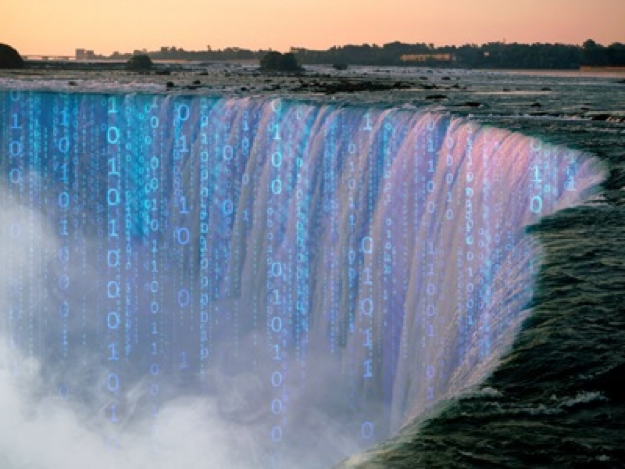
\includegraphics[width=1.0\textwidth]{bigdata}
\end{center}
\end{column}

\end{columns}
\end{frame}

%------------------------------------------------

\begin{frame}
\frametitle{Overcoming Data Scale: Data Streaming}


\begin{columns}
\begin{column}{0.55\textwidth}
	\begin{itemize}
		\item Traditional RAM algorithms scale poorly
		\begin{itemize}
			\item Awkward to store data in memory
			\item Superlinear scaling unacceptable
		\end{itemize}
		\item Data stream model to the rescue!
		\begin{itemize}
			\item Sequential data access
			\item Sublinear memory
			\item Linear amortized time
			\item Constrained number of passes
			\item Monte Carlo Approximations
		\end{itemize}
%		\item Increasingly want to 
%		\item \emph{Centrality} captures the ``importance'' of a vertex
%		\begin{itemize}
%			\item Many different measures
%			\item Expensive to recompute whenever graph changes
%		\end{itemize}
	%	\item Data warehousing becomes difficult
	%	\begin{itemize}
	%		\item parallelization, pass-contrained computation
	%	\end{itemize}
	\end{itemize}
\end{column}
\begin{column}{0.45\textwidth}  %%<--- here
\begin{center}
	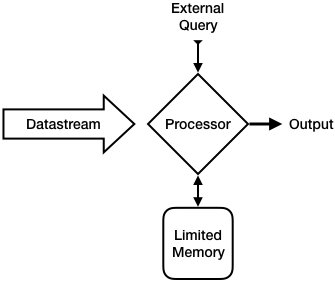
\includegraphics[width=1.0\textwidth]{stream_model}
\end{center}
\end{column}

\end{columns}
\end{frame}

%------------------------------------------------

\begin{frame}
\frametitle{Overcoming Data Scale: Distributed Data Streaming}


\begin{columns}
\begin{column}{0.65\textwidth}
	\begin{itemize}
		\item Distributed memory model a staple of HPC
		\begin{itemize}
			\item Divide computation across many processors
			\item Communication an important resource
			\item Immense scaling of exact algorithms
		\end{itemize}
		\item Why not distributed data streams!
		\begin{itemize}
			\item Sketch data structures afford stream composition
			\item Works nicely with vertex-centric algorithms
			\item Even greater scaling
			\item Linear communication
		\end{itemize}
%		\item Increasingly want to 
%		\item \emph{Centrality} captures the ``importance'' of a vertex
%		\begin{itemize}
%			\item Many different measures
%			\item Expensive to recompute whenever graph changes
%		\end{itemize}
	%	\item Data warehousing becomes difficult
	%	\begin{itemize}
	%		\item parallelization, pass-contrained computation
	%	\end{itemize}
	\end{itemize}
\end{column}
\begin{column}{0.35\textwidth}  %%<--- here
\begin{center}
	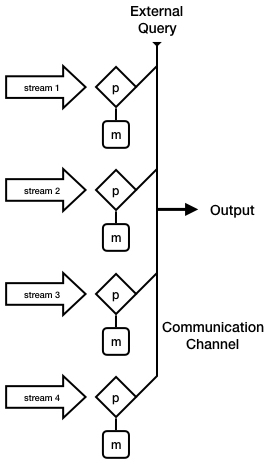
\includegraphics[width=0.9\textwidth]{dist_stream_model}
\end{center}
\end{column}

\end{columns}
\end{frame}

%------------------------------------------------

\begin{frame}
\frametitle{Centrality Indices}


\begin{columns}
\begin{column}{0.6\textwidth}
	\begin{itemize}
		\item Assign scores to vertices
		\begin{itemize}
			\item Higher score $\rightarrow$ more important
			\item Depends on graph structure
			\item Different indices in different domains
		\end{itemize}
		\item Scores are not informative
		\begin{itemize}
			\item Usually want top $k$ vertices
		\end{itemize}
		\item Relative order-preserving approximation is acceptable
	%	\item Data warehousing becomes difficult
	%	\begin{itemize}
	%		\item parallelization, pass-contrained computation
	%	\end{itemize}
	\end{itemize}
\end{column}
\begin{column}{0.4\textwidth}  %%<--- here
\begin{center}
	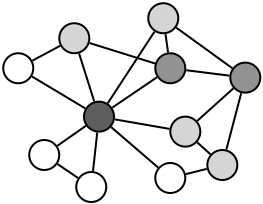
\includegraphics[width=1.0\textwidth]{centrality_greyscale}
\end{center}
\end{column}

\end{columns}
\end{frame}

%------------------------------------------------

 \begin{frame}
\frametitle{Large Scale Graph Centrality}

\textbf{The Problem}
\begin{itemize}
	\item Memory overhead
	\item Compuational Overhead
	\item Communication Overhead
	\item Wasted effort 
	\begin{itemize}
		\item Generally only need top elements vis-\'a-vis a centrality index
	\end{itemize}
\end{itemize}
\textbf{Our Solution}
\begin{itemize}
	\item Sketch data structures
	\begin{itemize}
		\item Utilize composable streaming summaries of vertex-local information
	\end{itemize}
	\item Distributed memory
	\begin{itemize}
		\item Partition graph and distribute sketches
		\item Polyloglinear computation, memory, and communication
	\end{itemize}
\end{itemize}

\end{frame}


%\begin{frame}
%\frametitle{Important Centrality Indices}
%
%
%\begin{itemize}
%	\item $O(n)$ space
%	\begin{itemize}
%		\item Degree Centrality
%	\end{itemize}
%	\vspace{-0.0cm}
%	\begin{equation*}
%		\textnormal{DC}(x) = |\{(u,v) \in E \mid x \in \{u,v\} \}| = \|A_{x,:}\|_1 = \|A_{:,x}\|_1
%%		\textnormal{IDC}(x) &= |\{(u,v) \in E \mid x=v\}| = \|A_{x,:}\|_1 \\
%%		\textnormal{ODC}(x) &= |\{(u,v) \in E \mid x=u\}| = \|A_{:,x}\|_1
%	\end{equation*}
%	\vspace{-0.7cm}
%	\item $O(m)$ space
%	\begin{itemize}
%		\item Closeness Centrality
%		\vspace{-0.1cm}
%		\begin{equation*}
%			\textnormal{CC}(x) = \frac{1}{\sum\limits_{y \in V} d(x,y)}
%		\end{equation*}
%		\vspace{-0.7cm}
%		\item Betweenness Centrality
%		\begin{equation*}
%			\textnormal{BC}(x) = \sum\limits_{\substack{x \not\in \{y,z\} \\ \lambda_{y,z} \neq 0}} \frac{\lambda_{y,z}(x)}{\lambda_{y,z}}
%		\end{equation*}
%		\item $\kappa$-Path Centrality
%		\vspace{-0.2cm}
%		\begin{equation*}
%			\textnormal{PC}(x, \kappa) = \Pr [x \in \text{ a random simple path of length $\leq \kappa$} ]
%		\end{equation*}
%		\item Eigencentrality
%		\vspace{-0.2cm}
%		\begin{equation*}
%			\textnormal{EC}(x) = u_{x} \text{, where $u$ is the dominant left eigenvector of $A$}
%		\end{equation*}
%	\end{itemize}
%\end{itemize}
%\end{frame}

%------------------------------------------------

%----------------------------------------------------------------------------------------
%----------------------------------------------------------------------------------------
\section{Background}
%----------------------------------------------------------------------------------------
%----------------------------------------------------------------------------------------


\begin{frame}
\frametitle{Graph Primitives}

Assume throughout that $\mathcal{G}=(\mathcal{V}, \mathcal{E}, \mathbf{w})$, where $|\mathcal{V}| = n$ and $|\mathcal{E}| = m$

\begin{itemize}
	\item $\mathbf{w}_e$ is the weight of edge $e$ if $e \in \mathcal{E}$ and zero otherwise
	\item $\mathcal{G}$ has adjacency matrix $A \in \mathbb{R}^{n \times n}$ so that $A_{x,y} = \textbf{w}_{xy}$ for $xy \in \mathcal{E}$
	\item $\mathcal{G}$ has vertex-edge incidence matrix $B \in \mathbb{R}^{{n \choose 2} \times n}$ so that 
$B_{xy,z} = 
\begin{cases}
\textbf{w}_{xy} & \textnormal{if $x=z$} \\
-\textbf{w}_{xy} & \textnormal{if $y=z$} \\
0 & \textnormal{else}.
\end{cases}$
\end{itemize}


\begin{columns}

\begin{column}{0.35\textwidth}
\begin{center}
\tikz \graph [nodes={draw,circle}] { a -- {b, c} -- d };
\end{center}
\end{column}

\begin{column}{0.65\textwidth}
\[
B=
\begin{blockarray}{ccccc}
& a & b & c & d \\
\begin{block}{c(cccc)}
  ab & 1 & -1 & 0 & 0 \\
  ac & 1 & 0 & -1 & 0 \\
  ad & 0 & 0 & 0 & 0 \\
  bc & 0 & 0 & 0 & 0 \\
  bd & 0 & 1 & 0 & -1 \\  
  cd & 0 & 0 & 1 & -1 \\
\end{block}
\end{blockarray}
 \]
\end{column}
\end{columns}

\end{frame}

%------------------------------------------------

\begin{frame}
\frametitle{Streaming Background}

\begin{itemize}
	\item A \emph{stream} $\sigma$ accumulating $\mathbf{f} \in \mathbb{R}^{n}$ is a list of rank-1 updates
	\begin{itemize}
		\item An update $(i,c)$ means $M \gets \mathbf{f} + c*e_i$
		\item A \emph{cash register} stream enforces $c > 0$ for all updates
		\item A \emph{turnstile} stream allows negative updates
		\item A \emph{strict turnstile} stream allows negatives but enforces $\mathbf{f} \in \mathbb{R}^{n}_{\geq 0}$
	\end{itemize}
	\item An algorithm accumulating a data structure $\mathcal{S}$ and is said to be...
	\begin{itemize}
		\item \emph{streaming} if $\mathcal{S}$ uses $O(\log n)$ memory
		\item \emph{semi-streaming} if $\mathcal{S}$ uses $O(n \polylog n)$\footnote{sometimes $O(n^{1+\alpha})$ for $\alpha \in (0,1/2]$} memory
	\end{itemize}
	\item Want to minimize the number of passes over $\sigma$	
	\begin{itemize}
		\item 1 pass ideal
		\item Constant or logarithmic passes sometimes acceptable 
	\end{itemize}

\end{itemize}

\end{frame}

%------------------------------------------------

\begin{frame}
\frametitle{Sketching}

\begin{definition}[Sketch]
A \emph{Sketch} is a streaming data structure $\mathcal{S}$ that admits a merge operator $\oplus$. 
If $\circ$ is the stream concatenation operator, then for any streams $\sigma_1$ and $\sigma_2$,
\begin{equation*}
	\mathcal{S}(\sigma_1) \oplus \mathcal{S}(\sigma_2) = \mathcal{S}(\sigma_1 \circ \sigma_2).
\end{equation*}
\end{definition}

\begin{definition}[Linear Sketch]
A \emph{Linear Sketch} $\mathcal{S}$ is a linear projection of $\mathbb{f}$ to a lower dimension.
For any streaming frequency vectors $\mathbf{f}_1$ and $\mathbf{f}_2$ and scalars $a$ and $b$, 
\begin{equation*}
	a\mathcal{S}(\mathbf{f}_1) + b\mathcal{S}(\mathbf{f}_2) = \mathcal{S}(a\mathbf{f}_1 + b\mathbf{f}_2).
\end{equation*}
\end{definition}

\begin{block}{}
\begin{center}
%	\vspace{-1.1em}
	Sketches are useful for stream summarization when \\
	\emph{comparisons between streams} are important
\end{center}
\end{block}

\end{frame}

%------------------------------------------------

\begin{frame}
\frametitle{Summary of Results: Serial Algorithms}

%Degree centrality
\begin{dynblock}
% First block
\opaqueblock<1->{
Degree Centrality
%
\vspace{-0.2cm}
%
\begin{equation*}
	\mathcal{C}^{\algoname{Deg}}(x) = |\{(u,v) \in E \mid x \in \{u,v\} \}| = \|A_{x,:}\|_1 = \|A_{:,x}\|_1
\end{equation*}
%
\vspace{-0.8cm}
%
\begin{itemize}
	\item Na\"ive online $O(n)$-space and -time algorithm exists
\end{itemize}
}

\invblock<2->

% Second block
\opaqueblock<2->[0.8\textwidth]{
\begin{center}
	\vspace{-1.1em}
	We show $\widetilde{O}(1)$-space distributable streaming algorithms
\end{center}
}
\end{dynblock}



%close/between centrality
\begin{dynblock}
% First block
\opaqueblock<3>{
Closeness Centrality
%
\vspace{-0.2cm}
%
\begin{equation*}
	\mathcal{C}^{\algoname{Close}}(x) = \frac{1}{\sum\limits_{y \in V} d(x,y)}
\end{equation*}
%
\vspace{-0.4cm}
%
\begin{itemize}	
	\item Online exact $O(n^2)$-space $O(nm)$-time algorithm \cite{wei2014real}
	\item Batch Approximate $O(n^2)$-space and almost-linear time algorithm \cite{cohen2014computing}
\end{itemize}
}

\invblock<4->

% Second block
\opaqueblock<4->[0.75\textwidth]{
\begin{center}
	\vspace{-1.1em}
	We show constant-pass semi-streaming algorithm
\end{center}
}

\end{dynblock}



%------------------------------------------------

\end{frame}

\begin{frame}
\frametitle{Summary of Results: Distributed Streaming Algorithms}

%Degree centrality
\begin{dynblock}
% First block
\opaqueblock<1->{
Triangle Count Centrality
%
\vspace{-0.2cm}
%
\begin{align*}
	\mathcal{C}^{\algoname{Tri}}(x) 
	&= |\{yz \in \mathcal{E} \mid xy, yz, xz \in \mathcal{E} \}| 
	& \textnormal{(vertex-local)} \\
	\mathcal{C}^{\algoname{Tri}}(xy) 
	&= |\{z \in \mathcal{E} \mid xy, yz, xz \in \mathcal{E} \}|
	& \textnormal{(edge-local)} \\	
\end{align*}
%
\vspace{-1.3cm}
%
\begin{itemize}
	\item Exact $O(m)$-space, $O(m^{\frac{3}{2}})$ serial and distributed algorithms \cite{arifuzzaman2013patric}
	\item Streaming sampling sublinear-space algorithms \cite{lim2015mascot, stefani2017triest}
	\begin{itemize}
		\item Including distributed generalizations \cite{shin2018tri, shin2018dislr, priest2018estimating}
	\end{itemize}
\end{itemize}
}

\invblock<2->

% Second block
\opaqueblock<2->[0.8\textwidth]{
\begin{center}
	\vspace{-1.1em}
	We show 2-pass, semi-streaming, distributed sketch-based query algorithms for estimating heavy hitters
\end{center}
}
\end{dynblock}


%close/between centrality
\begin{dynblock}
% First block
\opaqueblock<3>{
$\kappa$-Path Centrality
%
\vspace{-0.2cm}
%
\begin{equation*}
	\mathcal{C}^{\algoname{$\kappa$}}(x)  =  \Pr_{p: |p| \leq \kappa} [x \in p \wedge \text{$p$ a simple path } ]
\end{equation*}
%
\vspace{-0.6cm}
%
\begin{itemize}	
	\item $O(m)$-space $O(n^{1 + \alpha} \log^{2} n)$-time approximation algorithm \cite{wei2014real}
	\item Empirical proxy for betweenness centrality heavy hitters
	\begin{itemize}
		\item Online exact and approximate $O(n^2)$- and $O(m)$-space algorithms exist \cite{green2012fast, wei2014real, kourtellis2015scalable, bergamini2014approximating}%, [GMB12], [WC14], [KMB15], [BMS15]
	\end{itemize}
\end{itemize}
}

\invblock<4->

% Second block
\opaqueblock<4->[0.75\textwidth]{
\begin{center}
	\vspace{-1.1em}
	We show distributed sublinear vertex-centric sampling algorithm
\end{center}
}

\end{dynblock}







\end{frame}



%------------------------------------------------

%\begin{frame}
%\frametitle{Some Important Sketches}
%
%\begin{dynblock}
%% Tug-of-War
%\opaqueblock<1>{
%%
%\begin{tabular*}{\textwidth}{l @{\extracolsep{\fill}} r}
%\algoname{Tug-of-War} & \cite{alon1999space}%[AMS99]
%\end{tabular*}
%%
%\vspace{-0.5cm}
%%
%\begin{itemize}
%\item 4-universal hash function $h: [n] \rightarrow \{-1,1\}$
%\item Define $s \in \mathbb{R}^{n}$: $s^T = (h(1), \dots, h(n))$
%\item Accumulate $s^Tv$
%\end{itemize}
%}
%\invblock<2->
%
%% Second block
%\opaqueblock<2->[0.6\textwidth]{
%%
%\vspace{-0.5cm}
%%
%\begin{center}
%$(1\pm \varepsilon)$-approx of $F_2(v)$ w.h.p.
%\end{center}
%}
%%\invblock<5->
%%
%% Third block
%%\opaqueblock<5>[0.5\textwidth]{
%%%
%%\vspace{-0.3cm}
%%%
%%\begin{center}
%% $O \left ( \frac{\log(1/\delta)}{\varepsilon^{2}} (\log n + \log m) \right )$ space
%%\end{center}
%%}
%
%\end{dynblock}
%
%
%\begin{dynblock}
%% CountSketch
%\opaqueblock<3>{
%%
%\begin{tabular*}{\textwidth}{l @{\extracolsep{\fill}} r}
%\algoname{CountSketch} & \cite{charikar2002finding}%[CCFC04]
%\end{tabular*}
%%
%\vspace{-0.5cm}
%%
%\begin{itemize}
%\item 2-universal hash functions $h: [n] \rightarrow [r]$ and $s: [n] \rightarrow \{-1,1\}$
%\item Define $C \in \mathbb{R}^{r \times n}$: $C = \{0\}^{r \times n}$, $\forall j \in [n]$, $C_{h(j),j} = s(j)$
%\item Accumulate $Cv$
%\end{itemize}
%}
%%\invblock<2->
%\invblock<4->
%
%% Second block
%\opaqueblock<4->[0.7\textwidth]{
%Produce $\tilde{f}$ s.t. $\forall j \in [n]$, $|\tilde{f}(j) - v_j | \leq \varepsilon \|v_{-j}\|_2$ w.h.p.
%}
%%\invblock<5->
%%
%%% Third block
%%\opaqueblock<5>[0.3\textwidth]{
%%%
%%\vspace{-0.3cm}
%%%
%%\begin{center}
%%$O \left ( \frac{\log(n/\delta)}{\varepsilon^{2}} \right )$ space
%%\end{center}
%%}
%
%\end{dynblock}
%
%
%
%
%\begin{dynblock}
%% JLT
%\opaqueblock<5>{
%%
%\begin{tabular*}{\textwidth}{l @{\extracolsep{\fill}} r}
%Johnson-Lindenstrauss Transform (Gaussian variant) & \cite{har2012approximate} %[IM98]
%\end{tabular*}
%%
%\vspace{-0.5cm}
%%
%\begin{itemize}
%\item $R \in \mathbb{R}^{r \times n}$, where $R_i,j \sim \mathcal{N}(0,1)$ $\forall i,j$
%\item $S = \frac{1}{\sqrt{r}} R$
%\item Accumulate $Sv$
%\end{itemize}
%}
%%\invblock<2->
%\invblock<6->
%
%% Second block
%\opaqueblock<6>[0.6\textwidth]{
%$\forall v, v^\prime \in \mathbb{R}^n$:
%%
%\vspace{-0.3cm}
%%
%\begin{center}
%$\langle Sv, Sv^\prime \rangle - \langle v, v^\prime \rangle \leq \varepsilon \|v\|_2 \|v^\prime\|_2$ w.h.p.
%\end{center}
%}
%%\invblock<5->
%%
%%% Third block
%%\opaqueblock<5>[0.3\textwidth]{
%%%
%%\vspace{-0.3cm}
%%%
%%\begin{center}
%%$O \left ( \frac{\log(n/\delta)}{\varepsilon^{2}} \right )$ space
%%\end{center}
%%}
%
%\end{dynblock}
%
%
%
%\end{frame}

%------------------------------------------------



%\begin{frame}
%\frametitle{Important Applications}
%
%\begin{dynblock}
%% l2 sampling
%\opaqueblock<1>{
%%
%\begin{tabular*}{\textwidth}{l @{\extracolsep{\fill}} r}
%$\ell_p$-sampling & \cite{monemizadeh20101,jowhari2011tight}%[MW10], [JST11]
%\end{tabular*}
%%
%\vspace{-0.5cm}
%%
%\begin{itemize}
%\item Sample $t_i \sim_R (0,1)$ $\forall i \in [n]$
%\item Rescale updates to $v_i$ by $1/t_i^{1/p}$
%\item Accumulate \algoname{Tug-of-War}, \algoname{CountSketch}, and $\ell_p$-norm sketches
%\item Use sketches to output \algoname{CountSketch} argmax or FAIL
%\end{itemize}
%}
%\invblock<2->
%
%% Second block
%\opaqueblock<2->[0.6\textwidth]{
%%
%\vspace{-0.5cm}
%%
%\begin{center}
%Outputs $(i,P)$ w.h.p., where $i \in [n]$ is sampled w.p. $P = (1 \pm \varepsilon)\frac{|v_i|^p}{\|v\|^p_p}$ 
%\end{center}
%}
%%\invblock<3->
%%
%%% Second block
%%\opaqueblock<3->[0.7\textwidth]{
%%%
%%\vspace{-0.5cm}
%%%
%%\begin{center}
%%$O(\log^2n \log (1/\delta))$ space for $p=0$ \\
%%$O(\varepsilon^{-1}\log(1/\varepsilon)\log^2n \log (1/\delta))$ space for $p=1$ \\
%%\end{center}
%%}
%
%\end{dynblock}
%
%
%
%\begin{dynblock}
%% rank-k approximation
%\opaqueblock<3>{
%%
%\begin{tabular*}{\textwidth}{l @{\extracolsep{\fill}} r}
%Rank-$k$ Approximation (1-pass) & \cite{clarkson2009numerical}%[CW09]
%\end{tabular*}
%%
%\vspace{-0.5cm}
%%
%\begin{itemize}
%\item Given $A \in \mathbb{R}^{n \times d}$
%\item Sample JLTs $S \in \mathbb{R}^{(r/\varepsilon^2) \times n}$, $R \in \mathbb{R}^{d \times r}$
%\item Accumulate $SA$, $AR$, $SAR$
%\item Compute $U$, an orthonormal basis for the rowspace of $AR$
%\item Return $U[U^TAR(SAR)^+SA]_k$
%\end{itemize}
%}
%\invblock<4->
%
%% Second block
%\opaqueblock<4>[0.6\textwidth]{
%%
%\vspace{-0.5cm}
%%
%\begin{center}
%Outputs rank-$k$ factored $\tilde{A}_k$ s.t. $\|A - \tilde{A}_k \|_F \leq (1 + \varepsilon) \|A - A_k\|_F$ w.h.p.
%\end{center}
%}
%%\invblock<6>
%%
%%% Second block
%%\opaqueblock<6>[0.5\textwidth]{
%%%
%%\vspace{-0.5cm}
%%%
%%\begin{center}
%%$O(k\varepsilon^{-2}(n + d\varepsilon^{-2})\log (nd/\delta))$ space
%%\end{center}
%%}
%
%\end{dynblock}
%
%
%
%
%\end{frame}


%----------------------------------------------------------------------------------------
%----------------------------------------------------------------------------------------
%\section{Serial Streaming Algorithms}
%----------------------------------------------------------------------------------------
%----------------------------------------------------------------------------------------






%\begin{frame}
%\frametitle{Degree Centrality}
%
%\begin{columns}
%\begin{column}{0.5\textwidth}
%	\begin{itemize}
%		\item The degree centrality of a vertex is its valency
%		\item High degree-central vertices have many connections
%		\item Let $v \in \mathbb{R}^n$ be the vector of degree centralities
%		\begin{itemize}
%			\item $v_x$ is the row sum of $A_{x,:}$
%			\item $\sigma$ updating $A$ implicitly updates $v$
%		\end{itemize}
%	%	\item Data warehousing becomes difficult
%	%	\begin{itemize}
%	%		\item parallelization, pass-contrained computation
%	%	\end{itemize}
%	\end{itemize}
%\end{column}
%\begin{column}{0.5\textwidth}  %%<--- here
%\begin{center}
%	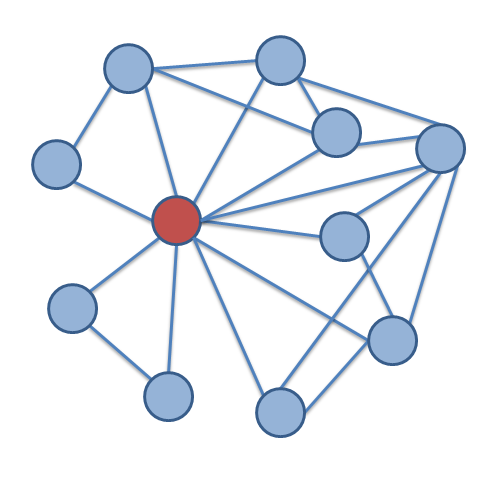
\includegraphics[width=1.0\textwidth]{centrality}
%\end{center}
%\end{column}
%
%\end{columns}
%\end{frame}

%------------------------------------------------

%\begin{frame}
%\frametitle{\algoname{CountSketch}}
%
%\begin{columns}
%\begin{column}{0.65\textwidth}
%	\begin{itemize}
%		\item Consider 2-universal hash functions
%		\begin{itemize}
%			\item $h_1, \dots, h_t : [n] \rightarrow [r]$
%			\item $s_1, \dots, s_t : [n] \rightarrow \{-1,1\}$
%		\end{itemize}
%		\item Define $C^{(i)} \in \mathbb{R}^{r \times n}$:
%		\begin{itemize}
%			\item $C^{(i)}_{h(j),j} \gets s(j)$ for each $j \in [n]$
%		\end{itemize}
%		\item $(C^{(i)}v)_x*s(x)$ is a good estimator for $v_x$
%		\item $\med_{i \in [t]} \{(C^{(i)}v)_x*s_i(x) \}$ has low variance
%	%	\item Data warehousing becomes difficult
%	%	\begin{itemize}
%	%		\item parallelization, pass-contrained computation
%	%	\end{itemize}
%	\end{itemize}
%\end{column}
%\begin{column}{0.35\textwidth}  %%<--- here
%\begin{center}
%	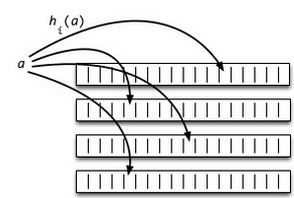
\includegraphics[width=1.0\textwidth]{CS}
%\end{center}
%\end{column}
%
%\end{columns}
%
%
%\begin{theorem}[\algoname{CountSketch}]
%%Let $v \in \mathbb{R}^n$ and $C_1, \dots, C_t \in \mathbb{R}^{r \times n}$ be \algoname{CountSketch} matrices.
%For every $j \in n$ let $\tilde{v}_j = \med_{i \in [t]} \{(C^{(i)}v)_{h(j)} * s_i(j)\}$.
%If $r= O(\varepsilon^{-2})$ and $t=O(\log(1/\delta))$, then for all $j \in [n]$ with probability at least $1-\delta$:
%%
%\begin{equation*}
%|\tilde{v}_j - v_j | \leq \varepsilon \|v_{-j}\|_2
%\end{equation*}
%%
%
%\end{theorem}
%
%\end{frame}

%------------------------------------------------

%\begin{frame}
%\frametitle{Approximating the Top $k$ Degree Centralities}
%
%\begin{definition}[\algoname{FindApproxTop}$(\sigma, k, \varepsilon)$]
%Given $\sigma$ updating $v \in \mathbb{R}^n$, $k < n$, and $\varepsilon \in \mathbb{R}^+$, output a list of $k$ indices of $v$ so that for each such index $j \in [n]$, $v_j > (1-\varepsilon)v_\ell$, where $v_\ell$ is the $k$th-largest index of $v$.
%\end{definition}
%
%\begin{itemize}
%	\item \cite{charikar2002finding} gives an algorithm using \algoname{CountSketch} that solves \algoname{FindApproxTop}$(\sigma, k, \varepsilon)$ by maintaining a heap while accumulating $C$
%	\begin{itemize}
%		\item Uses space $O \left (k \log \frac{n}{\delta} + \frac{\sum_{q = k+1}^n n_q^2}{n_k^2} \varepsilon^{-2} \log \frac{n}{\delta} \right )$ \footnote{$n_q$ is the value of the $q$th largest index of $v$}
%	\end{itemize}
%	\item Immediately applicable to degree centrality
%	\item $O((k + \varepsilon^{-2})\log (n/\delta))$ memory for strongly non-regular graphs
%\end{itemize}
%
%\end{frame}

%------------------------------------------------


%------------------------------------------------

%------------------------------------------------
%\section{Multi-Pass Semi-Streaming Closeness Centrality}
%------------------------------------------------

%------------------------------------------------

%\begin{frame}
%\frametitle{Closeness Centrality}
%
%\begin{columns}
%\begin{column}{0.6\textwidth}
%	\begin{itemize}
%		\item For vertex $x$, $CC(x) = \frac{1}{\sum_{y \in V} d(x,y)}$
%		\item High closeness-central vertices have short paths to the rest of the graph
%		\item Solving exactly requires solving \algoname{All Pairs Shortest Paths}
%		\item We solve approximately using a graph spanner obtained via $\ell_1$-sparsification on $B$, $G$'s node-edge incidence matrix
%	%	\item Data warehousing becomes difficult
%	%	\begin{itemize}
%	%		\item parallelization, pass-contrained computation
%	%	\end{itemize}
%	\end{itemize}
%\end{column}
%\begin{column}{0.4\textwidth}  %%<--- here
%\begin{center}
%	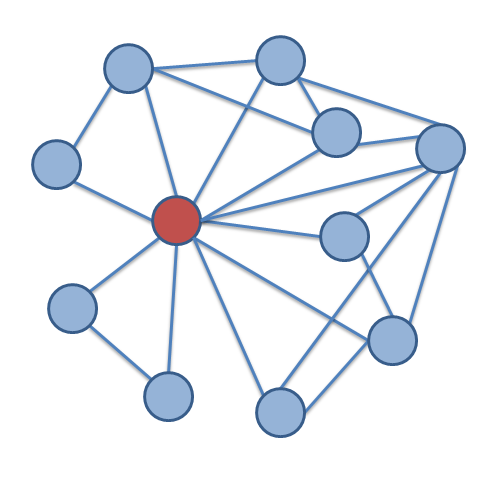
\includegraphics[width=1.0\textwidth]{centrality}
%\end{center}
%\end{column}
%
%\end{columns}
%\end{frame}

%------------------------------------------------

%----------------------------------------------------------------------------------------
%----------------------------------------------------------------------------------------
%\section{Semi-Streaming Closeness Centrality}
%----------------------------------------------------------------------------------------
%----------------------------------------------------------------------------------------




%\begin{frame}
%\frametitle{Closeness Centrality Approximation}
%
%
%\begin{definition}[$\alpha$-Spanner]
%A subgraph $H$ of $G$ such that $d_H(x,y) \leq \alpha d_G(x,y)$ for every $x,y \in V$
%\end{definition}
%
%\begin{itemize}
%	\item A sampling algorithm produces a graph spanner \cite{ahn2012graph}:
%	\begin{itemize}
%		\item Produces a $(k^{\log_2 5} - 1)$-spanner
%		\item Requires $O(n^{1+1/k})$ space
%		\item Requires $\log k$ passes
%	\end{itemize}
%	\item Trades off estimation accuracy for reduced space and passes
%	\item Can compute closeness centrality on $H$!
%\end{itemize}
%
%\end{frame}

%------------------------------------------------


%\begin{frame}
%\frametitle{Closeness Centrality Approximation, continued}
%
%
%\begin{itemize}
%	\item If $H$ is an $\alpha$-spanner of $G$, then
%{\footnotesize
%\begin{align*}
%CC_H(x) 
%= \frac{1}{\sum\limits_{y \in V} d_H(x,y)}
%\geq \frac{1}{\sum\limits_{y \in V} \alpha d_G(x,y)}
%= \frac{1}{\alpha}CC_G(x)
%\end{align*}
%}
%	\item Thus, $CC_H(x) \in \left [\frac{1}{\alpha}, 1 \right ] CC_G(x)$
%	\item \algoname{AllPairsShortestPaths} more efficient on $H$ than $G$
%	\begin{itemize}
%		\item Especially if $G$ is dense
%	\end{itemize}
%	\item Some weaknesses
%	\begin{itemize}
%		\item $\tilde{O}(n^{1+1/k})$ rather than $O(n \polylog n)$ space
%		\item No top-$k$ preservation guarantees
%		\item Greatest improvement when $G$ is dense
%		\item Not suitable for online applications
%	\end{itemize}
%\end{itemize}
%
%\end{frame}

%------------------------------------------------







%------------------------------------------------

%------------------------------------------------
%\section{Discussion of Betweenness Centrality}
%------------------------------------------------

%------------------------------------------------

%\begin{frame}
%\frametitle{Betweenness Centrality}
%
%\begin{columns}
%\begin{column}{0.7\textwidth}
%	\begin{itemize}
%		\item For $x,y,z \in V$, let $\lambda_{y,z}$ and $\lambda_{y,z}(x)$ be the number of shortest paths from $y$ to $z$ and the number which pass through $x$, respectively
%		\item For vertex $x$, $BC(x) = \sum\limits_{\substack{x \not\in \{y,z\} \\ \lambda_{y,z} \neq 0}} \frac{\lambda_{y,z}}{\lambda_{y,z}(x)}$
%		\item High betweenness-central vertices connect groups of vertices to others
%		\item Solving exactly requires solving \algoname{All Pairs All Shortest Paths}
%		\begin{itemize}
%			\item Strictly more difficult than \algoname{All Pairs Shortest Paths}
%			\item Spanner-based approach will not work
%		\end{itemize}
%		\item Many algorithms solve or approximate BC in evolving graphs, but none use sublinear memory
%	%	\item Data warehousing becomes difficult
%	%	\begin{itemize}
%	%		\item parallelization, pass-contrained computation
%	%	\end{itemize}
%	\end{itemize}
%\end{column}
%\begin{column}{0.3\textwidth}  %%<--- here
%\begin{center}
%	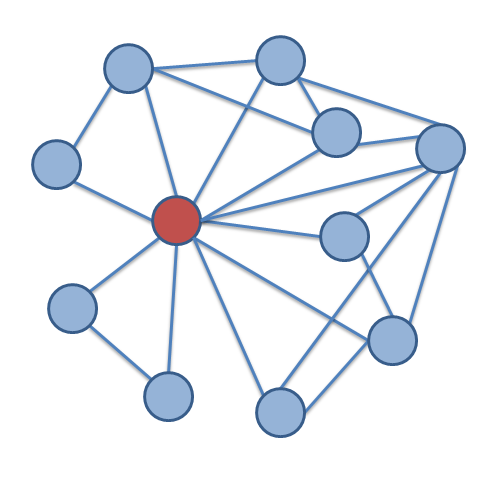
\includegraphics[width=1.0\textwidth]{centrality}
%\end{center}
%\end{column}
%
%\end{columns}
%\end{frame}
%
%%------------------------------------------------
%
%\begin{frame}
%\frametitle{A Proxy: $\kappa$-path centrality}
%
%
%\begin{definition}[$\kappa$-Path Centrality]
%For $x \in V$, $PC_\kappa(x)$ is the sum of probabilities over all $y \in V \setminus \{x\}$ that a random simple path originating at $y$ passes through $x$. 
%\end{definition}
%
%\begin{itemize}
%	\item $PC_\kappa(x)$ has been shown to correlate with $BC(x)$ in real networks for $x$ with relatively high $BC(x)$
%	\begin{itemize}
%		\item No absolute error guarantees
%	\end{itemize}
%	\item Existing approximation algorithms $\kappa$-path centrality assume a static graph
%	\item May be approximable using $\ell_1$-graph sparsification techniques
%\end{itemize}
%
%\begin{block}{}
%This approach warrants further study
%\end{block}
%
%\end{frame}

%------------------------------------------------







%------------------------------------------------

%------------------------------------------------
%\section{Spectral Centrality and A Semi-Streaming \algoname{HITS} approximation}
%------------------------------------------------

%------------------------------------------------

%\begin{frame}
%\frametitle{Spectral Measures of Centrality}
%
%\begin{itemize}
%	\item We will call any centrality measure that relies on the eigenvalues or eigenvectors of a matrix derived from $G$ \emph{spectral}
%	\begin{itemize}
%		\item e.g. Katz's index, PageRank, \algoname{HITS}, SALSA
%		\item Most require only dominant eigenvector
%	\end{itemize}
%	\item Sketching is useful for numerical linear algebra, though best results are on ``tall'' matrices
%	\item Many different semi-streaming low-rank approximations
%	\begin{itemize}
%		\item Produce factorizations similar to rank-$r$ SVD
%	\end{itemize}
%	\item Can learn the eigenvector of a rank-1 approximation so obtained
%	\begin{itemize}
%		\item However, no error guarantees
%		\item No simple way to maintain ``top $k$'' vertices
%	\end{itemize}
%\end{itemize}
%
%\end{frame}

%------------------------------------------------


%----------------------------------------------------------------------------------------
%----------------------------------------------------------------------------------------
%\section{Semi-Streaming Parallel HITS}
%----------------------------------------------------------------------------------------
%----------------------------------------------------------------------------------------


%\begin{frame}
%\frametitle{Approximating \algoname{HITS}}
%
%\begin{itemize}
%	\item \algoname{HITS} is a variant of eigencentrality producing two symbiotic scores
%	\begin{itemize}
%		\item authoritativeness: sites that are linked by hubby sites
%		\item hubbiness: sites that link to authoritative sites
%	\end{itemize}
%	\item Authoritativeness and Hubbiness converge to left dominant eigenvectors of $A^TA$ and $AA^T$, respectively
%	\begin{itemize}
%		\item If $A=U\Sigma V^T$ is the SVD, then $A^TA = V\Sigma^2V^T$ and $AA^T = U\Sigma^2U^T$
%	\end{itemize}
%	\item There is an algorithm for approximating the right singular vectors of a matrix \cite{anaraki2014memory}%[GPW12]
%	\begin{itemize}
%		\item Straightforward algorithm relying on JLTs
%	\end{itemize}
%\end{itemize}
%
%
%\begin{dynblock}
%% rank-k approximation
%\opaqueblock<2>{
%%
%Let $A = U \Sigma V^T$ be the $r$-truncated SVD of rank-$r$ $A \in \mathbb{R}^{n \times d}$. 
%Then w.h.p. the algorithm of [GPW12] returns $\tilde{V}$ so that
%\begin{equation*}
%\| V_{:,j} - \tilde{V}_{:,j}\|_2 \leq 
%\min 
%\left \{ 
%\sqrt{2}, 
%\frac{\varepsilon \sqrt{1+ \varepsilon}}{\sqrt{1-\varepsilon}}
%\max\limits_{i\neq j}
%\frac{\sqrt{2}\Sigma_{i,i} \Sigma_{j,j}}
%%{}
%{\min\limits_{c \in [-1,1]} \{| \Sigma_{i,i}^2 - \Sigma_{j,j}^2 (1 + c\varepsilon)|\}}
%\right \}
%\end{equation*}
%}
%\invblock<3->
%
%% Second block
%\opaqueblock<3>[0.6\textwidth]{
%%
%\vspace{-0.5cm}
%%
%\begin{center}
%$O(nr\varepsilon^{-2}(\log (1/\varepsilon) + \log (1/\delta)))$ space
%\end{center}
%}
%%\invblock<3->
%
%\end{dynblock}
%
%
%%\begin{theorem}[Singular Vector Approximation {[GPW12]}]
%%Let $A = U \Sigma
%%%\begin{equation*}
%%%\| V_j - V^\prime_j\|_2 = 
%%%\min 
%%%\left \{ 
%%%\sqrt{2}, 
%%%\frac{\varepsilon \sqrt{1+ \varepsilon}}{\sqrt{1-\varepsilon}}
%%%\max\limits_{i\neq j}
%%%\frac{\sqrt{2}\sigma_i \sigma_j}
%%%%{}
%%%{\min\limits_{c \in [-1,1]} \{| \sigma_i^2 - \sigma_j^2 (1 + c\varepsilon)|\}}
%%%\right \}
%%%\end{equation*}
%%%%
%%%Here $\sigma_j$ is the $j$th singular value of $A$, and $\varepsilon$ is a given accuracy parameter
%%\end{theorem}
%
%\end{frame}
%
%%------------------------------------------------
%
%\begin{frame}
%\frametitle{Approximating \algoname{HITS}, continued}
%
%\begin{itemize}
%	\item \cite{anaraki2014memory} prompts a \algoname{HITS} approximation algorithm
%	\begin{itemize}
%		\item Approximate $r$-truncated left singular vectors $\tilde{V}$ of $A$ and $\tilde{U}$ of $A^T$
%		\item Set $\tilde{C}_{\textnormal{auth}}(x) = \tilde{V}_{1,x}$ and $\tilde{C}_{\textnormal{hub}}(x) = \tilde{U}_{1,x}$
%		\item Single Pass!
%		\item Bounded error on individual vertices!
%%	    	\item Requires $O(nr\varepsilon^{-2}(\log (1/\varepsilon) + \log (1/\delta)))$ space, where $\algoname{rank}(A) = r$
%	\end{itemize}
%	\item Some weaknesses
%	\begin{itemize}
%		\item Loose bound, especially when $A$'s singular values are close together
%    		\item Only efficient on highly disconnected graphs
%	\end{itemize}
%	\item Any approximation of the top singular vector of a square matrix with error $\leq \frac{1}{2}$  requires $\Omega(n^{3/2})$ space \cite{li2014sketching}
%%	\begin{itemize}
%%		\item Cannot do much better
%%	\end{itemize}
%\end{itemize}
%
%\end{frame}

%------------------------------------------------








%----------------------------------------------------------------------------------------
%----------------------------------------------------------------------------------------
\section{Pseudo-Asynchronous Communication Schemes for Vertex-Centric Distributed Algorithms}
%----------------------------------------------------------------------------------------
%----------------------------------------------------------------------------------------

\begin{frame}
\frametitle{Motivation: Vertex-Centric Algorithms}

\textbf{The Problem}:
\begin{itemize}
	\item Most distributed graph algorithms are vertex-centric
	\begin{itemize}
		\item Partition local vertex information across processors
		\item Processors communicate as in rounds \cite{malewicz2010pregel}
	\end{itemize}
	\item Scale-free graphs common in applications
	\begin{itemize}
		\item Exhibit very high degree vertices
		\item Cause computation, communication, and memory ``hotspots''
		\item Synchronous communication moves at the speed of the slowest processor
	\end{itemize}
\end{itemize}

\textbf{Existing Solutions}:
\begin{itemize}
	\item Asynchronous Communication 
	\begin{itemize}
		\item Processors communicate point-to-point as needed
		\item Increased implementation complexity
	\end{itemize}
	\item Vertex delegation \cite{pearce2014faster}
	\begin{itemize}
		\item Subpartition high degree vertices between processors
		\item Adds communication overhead
	\end{itemize}
\end{itemize}


\end{frame}

%----------------------------------------------------------------------------------------

\begin{frame}
\frametitle{Approach: Pseudo-Asynchronous Communication Protocol}

\begin{block}{The Idea}
Allow processors to drop out of communication exchanges when finished
\end{block}

\begin{itemize}
	\item Partion processor set $\mathcal{P}$ into \emph{local} and \emph{remote} exchanges
	\begin{itemize}
%		\item Each processor belongs to one local and one remote exchange
		\item Takes advantage of hybrid distributed memory
	\end{itemize}
	\item $P \in \mathcal{P}$ maintains send buffer $\mathcal{S}[P]$ and receive buffer $\mathcal{R}[P]$ 
	\begin{itemize}
		\item Begin forwarding messages when $\mathcal{S}[P]$ reaches threshold
		\item Drop out of exchange when all other processors in exchanges stop updating $\mathcal{R}[P]$
	\end{itemize}
	\item Three protocols:
	\begin{itemize}
		\item Node Local
		\item Node Remote
		\item Node Local Node Remote (NLNR)
	\end{itemize}
\end{itemize}

\end{frame}

%----------------------------------------------------------------------------------------

\begin{frame}
\frametitle{Node Local and Node Remote}


\begin{columns}
\begin{column}{0.65\textwidth}
	\textbf{Node Local}
	\begin{enumerate}
		\item Send messages to local core matching destination local offset
		\item Send messages to remote core matching destination node offset
		\item Good for mostly point-to-point messages
	\end{enumerate}
	\textbf{Node Remote}
	\begin{enumerate}
		\item Send messages to remote core matching destination node offset
		\item Send messages to local core matching destination local offset
		\item Good for large numbers of broadcasts
	\end{enumerate}
\end{column}
\begin{column}{0.35\textwidth}  %%<--- here
\begin{center}
	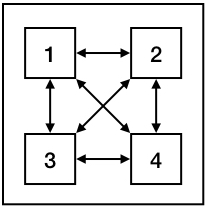
\includegraphics[width=0.7\textwidth]{local}
\end{center}
\begin{center}
	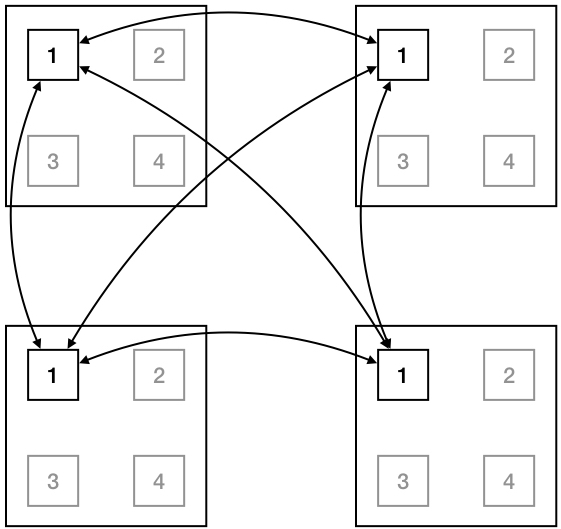
\includegraphics[width=1.0\textwidth]{remote}
\end{center}
\end{column}

\end{columns}

\end{frame}

%----------------------------------------------------------------------------------------

\begin{frame}
\frametitle{Node Local Node Remote}


\begin{columns}
\begin{column}{0.7\textwidth}
	\textbf{Node Local Node Remote}
	\begin{itemize}
		\item Further partition processors by \emph{layers}
		\begin{itemize}
			\item A layer is a collection of nodes equal to the number of cores per node
		\end{itemize}
	\end{itemize}
	\begin{enumerate}
		\item Send messages to local core matching destination layer offset
		\item Send messages to remote core matching destination node offset
		\item Send messages to local core matching destination local offset
		\item Best for extreme scale where many layers exist
	\end{enumerate}
\end{column}
\begin{column}{0.3\textwidth}  %%<--- here
\begin{center}
	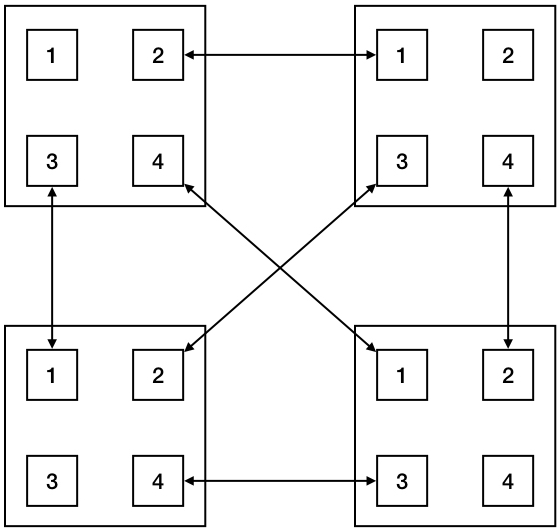
\includegraphics[width=1.0\textwidth]{intra_layer_nlnr}
\end{center}
\begin{center}
	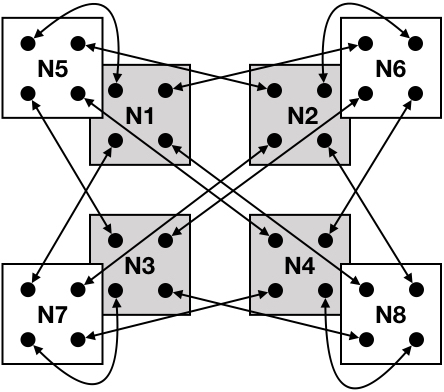
\includegraphics[width=1.0\textwidth]{inter_layer_nlnr}
\end{center}
\end{column}

\end{columns}

\end{frame}

%----------------------------------------------------------------------------------------

\begin{frame}
\frametitle{Validation of Claims}


\begin{columns}
\begin{column}{0.3\textwidth}
	\textbf{Experiment}
	\begin{itemize}
		\item 20B message exchange
		\begin{itemize}
			\item Destination sampled from Pareto distribution
			\item Batch size is maximum $|\mathcal{S}[P]|$
		\end{itemize}
	\end{itemize}
\end{column}
\begin{column}{0.7\textwidth}  %%<--- here
\begin{center}
	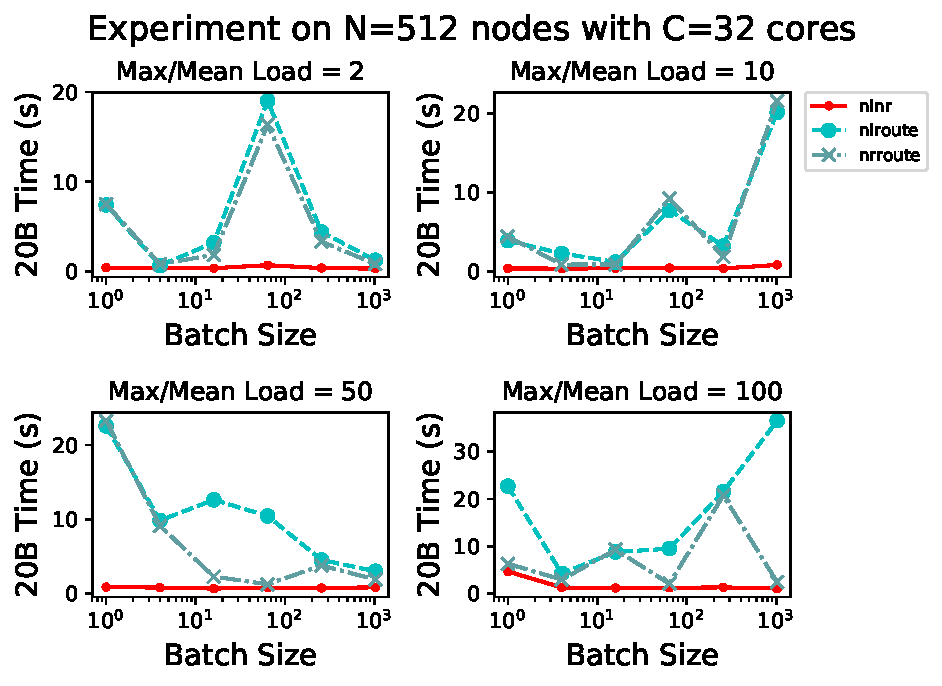
\includegraphics[width=1.0\textwidth]{512_32}
\end{center}
\end{column}

\end{columns}

\begin{block}{}
	\begin{center}
		NLNR exhibits best scaling, others more useful with fewer nodes
	\end{center}
\end{block}

\end{frame}

%----------------------------------------------------------------------------------------

\begin{frame}
\frametitle{Implementation Details}


\textbf{\algoname{YGM} C++/MPI Library}
\begin{itemize}
	\item Authored by myself, Trevor Steil (UMN), and Roger Pearce (LLNL)
	\item Simple API for handling pseudo-asynchronous communication
	\begin{itemize}
		\item Clients need only specify receive behavior
	\end{itemize}
	\item Supports message serialization for arbitrary, variable-length messages
	\item Supports LLNL Projects
	\begin{itemize}
		\item HAVOQgt
		\item graph500 scale leader
		\item others?
	\end{itemize}
	\item Useful for not just vertex-centric algorithms, but any algorithm with asymmetric computational and communication load
\end{itemize}

\begin{block}{}
	\begin{center}
		\algoname{YGM} to be open sourced	
	\end{center}
\end{block}

\end{frame}


%----------------------------------------------------------------------------------------
%----------------------------------------------------------------------------------------
\section{\algoname{DegreeSketch} and Local Triangle Count Heavy Hitters}
%----------------------------------------------------------------------------------------
%----------------------------------------------------------------------------------------

\begin{frame}
\frametitle{Motivation: Local Triangle Counting}

\textbf{The Problem}:
\begin{itemize}
	\item Local triangle counting a common big data analytic
	\begin{itemize}
		\item Exact computation expensive $O \left ( m^{\frac{3}{2}} \right )$!
	\end{itemize}
	\item Recall
\end{itemize}
%
\vspace{-0.5em}
\begin{align*}
	\mathcal{C}^{\algoname{Tri}}(x) 
	&= |\{yz \in \mathcal{E} \mid xy, yz, xz \in \mathcal{E} \}| 
	& \textnormal{(vertex-local)} \\
	\mathcal{C}^{\algoname{Tri}}(xy) 
	&= |\{z \in \mathcal{E} \mid xy, yz, xz \in \mathcal{E} \}|
	& \textnormal{(edge-local)} 
\end{align*}
%\vspace{-1.0em}
%
\textbf{Existing Solutions}:
\begin{itemize}
	\item Many exact distributed algorithms \cite{arifuzzaman2013patric, pearce2017triangle}
	\item Many approximate streaming algorithms via sampling \cite{lim2015mascot, stefani2017triest}
	\item ... and some utilizing both models \cite{shin2018tri, shin2018dislr}
\end{itemize}


\end{frame}

%----------------------------------------------------------------------------------------

\begin{frame}
\frametitle{Approach: Sublinear Intersection Method}


\begin{columns}
\begin{column}{0.65\textwidth}
	\textbf{Idea}: Intersection method, but using cardinality sketches
	\begin{itemize}
		\item Cardinality sketches summarize set size
		\item Support union operation, and some support limited intersection operation
		\begin{itemize}
			\item High variance if intersection is small
			\item Likely best performance on heavy hitters
		\end{itemize}
		\item Affords edge- and vertex-local triangle count estimation
		\item Outputs only reliable if \emph{triangle density} is nontrivial
		\begin{itemize}
			\item Triangle density = $\frac{\textnormal{\# triangles}}{\textnormal{\# possible triangles}}$
		\end{itemize}
	\end{itemize}
\end{column}
\begin{column}{0.35\textwidth}  %%<--- here
	\begin{center}
		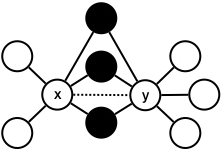
\includegraphics[width=1.0\textwidth]{edge_local}
	\end{center}
	\begin{center}
		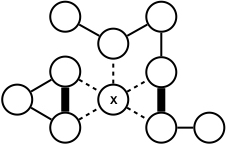
\includegraphics[width=1.0\textwidth]{vertex_local}
	\end{center}
\end{column}

\end{columns}


\end{frame}


%----------------------------------------------------------------------------------------

\begin{frame}
\frametitle{\algoname{HyperLogLog} Cardinality Sketches}

\begin{dynblock}
% l2 sampling
\opaqueblock<1>{
%
\textbf{\algoname{HLL} cardinality sketches} \\
Maintain $r = 2^p$ 6-bit registers $M$ and a 64-bit hash function $h$
\begin{itemize}
\item Insert $x$: let $i = \langle x_1, \dots, x_p \rangle$ and $w = \langle x_{p+1}, \dots, x_{64} \rangle$ 
\item $\rho(w) = $ initial zero bits of $w$ plus 1
\item $M_i = \max \{ M_i, \rho(w) \}$
\item Estimator derives from harmonic mean of $M$
\end{itemize}
%
}
\invblock<2->

% Second block
\opaqueblock<2->[0.6\textwidth]{
%
\vspace{-0.5cm}
%
\begin{center}
Outputs $\widetilde{C}$ such that for cardinality C, w.h.p. $| C - \widetilde{C} | \leq \frac{1.04}{\sqrt{m}} C$ \cite{flajolet2007hyperloglog}
\end{center}
}
\end{dynblock}



\begin{dynblock}
% rank-k approximation
\opaqueblock<3>{
%
\begin{tabular*}{\textwidth}{l @{\extracolsep{\fill}} r}
\textbf{Useful results}  & 
%[CW09]
\end{tabular*}
%
\vspace{-0.5cm}
%
\begin{itemize}
	\item Native intersection operator (elementwise maximum)
	\item Various improved harmonic \cite{heule2013hyperloglog, qin2016loglog} and maximum likelihood estimators \cite{xiao2017better, lang2017back, ertl2017new}
	\item Sparsification for low cardinality sets \cite{heule2013hyperloglog}
	\item Compression to 4 and 3 bit registers \cite{xiao2017better}
	\item Intersection estimators \cite{ting2016towards, cohen2017minimal, ertl2017new}
\end{itemize}
}

\end{dynblock}




\end{frame}


%----------------------------------------------------------------------------------------



\begin{frame}
\frametitle{\algoname{DegreeSketch} and Triangle Counting}


%\begin{definition}[$\ell_p$-Sampling Sketch]
%A distribution $\Pi$  on $k \times n$ matrices so that if for any $v \in \mathbb{R}^n$, $S$ drawn from $\Pi$ is such that, given $Sv$, one can produce $i \in [n]$ sampled with probability $(1 \pm \varepsilon)\frac{|v_i|^p}{\|v\|_p}$
%\end{definition}

Assume a partition $f : \mathcal{V} \rightarrow \mathcal{P}$, and let $\mathcal{V}_P = \{v \in \mathcal{V} \mid f(v) = P\}$
\begin{itemize}
	\item Distribute $\algoname{DegreeSketch}$ $\mathcal{D}$ across $\mathcal{P}$
	\begin{itemize}
		\item $\mathcal{D}[v]$ holds a \algoname{HLL} for adjacency set of $v \in \mathcal{V}$
		\item $P$ holds $\mathcal{D}[v]$ for $v \in \mathcal{V}_P$
	\end{itemize}
	\item Accumulate $\mathcal{D}$ in one pass over $\sigma$
	\begin{itemize}
		\item Assume $P \in \mathcal{P}$	gets substream $\sigma_P$
		\item $P$ sends $xy \in \sigma_P$ to $f(x)$ and $f(y)$
		\item When $P$ gets $xy : x \in \mathcal{V}_P$, insert $y$ into $\mathcal{D}[x]$
		\begin{itemize}
			\item $\mathcal{D}[x]$ starts sparse and eventually saturates
		\end{itemize}
	\end{itemize}
	\item $\mathcal{D}$ can be queried after estimation, e.g.
	\begin{itemize}
		\item Estimate $\widetilde{\mathcal{C}}^{\algoname{Deg}}(v)  = \algoname{Estimate}(\mathcal{D}[v])$
		\item Estimate $\widetilde{\mathcal{C}}^{\algoname{Tri}}(uv) = \mathcal{D}[u] \widetilde{\cap} \mathcal{D}[v]$
		\begin{itemize}
			\item Involves communication if $f(u) \neq f(v)$
		\end{itemize}
		\item Estimate $\widetilde{\mathcal{C}}^{\algoname{Tri}}(v) = \frac{\sum_{uv \in \mathcal{E}} \widetilde{\mathcal{C}}^{\algoname{Tri}}(uv)}{2}$
		\begin{itemize}
			\item Requires second pass in general
		\end{itemize}
	\end{itemize}
\end{itemize}

\begin{block}{}
\begin{center}
$\widetilde{O}(m)$ time and communication and $\widetilde{O}(\varepsilon^{-2}n)$ space!
\end{center}
\end{block}

\end{frame}

%----------------------------------------------------------------------------------------

\begin{frame}
\frametitle{Edge-Local Triangle Count Heavy Hitters}

\begin{algorithm}[H]
\caption{Edge-Local Triangle Count Heavy Hitters}\label{alg:sublinear_kpath}
\begin{algorithmic}[1]
%\State $T \gets 2 \kappa^2 n^{1-2\alpha} \ln n$
\State Accumulate $\mathcal{D}$ in distributed pass over $\sigma$
\State $H_k \gets \textnormal{empty $k$-heap}$
\State $T \gets 0$
\ParFor{$xy \in \sigma_P$}  \qquad // second pass
	\State Send $(\textnormal{E}, xy)$ to $f(x)$ and $(\textnormal{E}, yx)$ $f(y)$
	\For {$(\textnormal{E}, xy) \in \mathcal{R}[P]$}
		\State Send $(\textnormal{S}, xy, \mathcal{D}[x])$ to $f(y)$
	\EndFor
	\For {$(\textnormal{S}, xy, \mathcal{D}[x]) \in \mathcal{R}[P]$}
		\State Insert $(xy, \mathcal{D}[x] \widetilde{\cap} \mathcal{D}[y])$ into $H_k$
		\State $T \gets T + \mathcal{D}[x] \widetilde{\cap} \mathcal{D}[y]$
	\EndFor
\EndParFor
\State $T \gets T / 2$
\State Global accounting of $T$, $H_k$
\State \Return $H_k$
\end{algorithmic}
\end{algorithm}



\end{frame}


%----------------------------------------------------------------------------------------

\begin{frame}
\frametitle{Validation of Claims: Precision and Recall}

\centerline{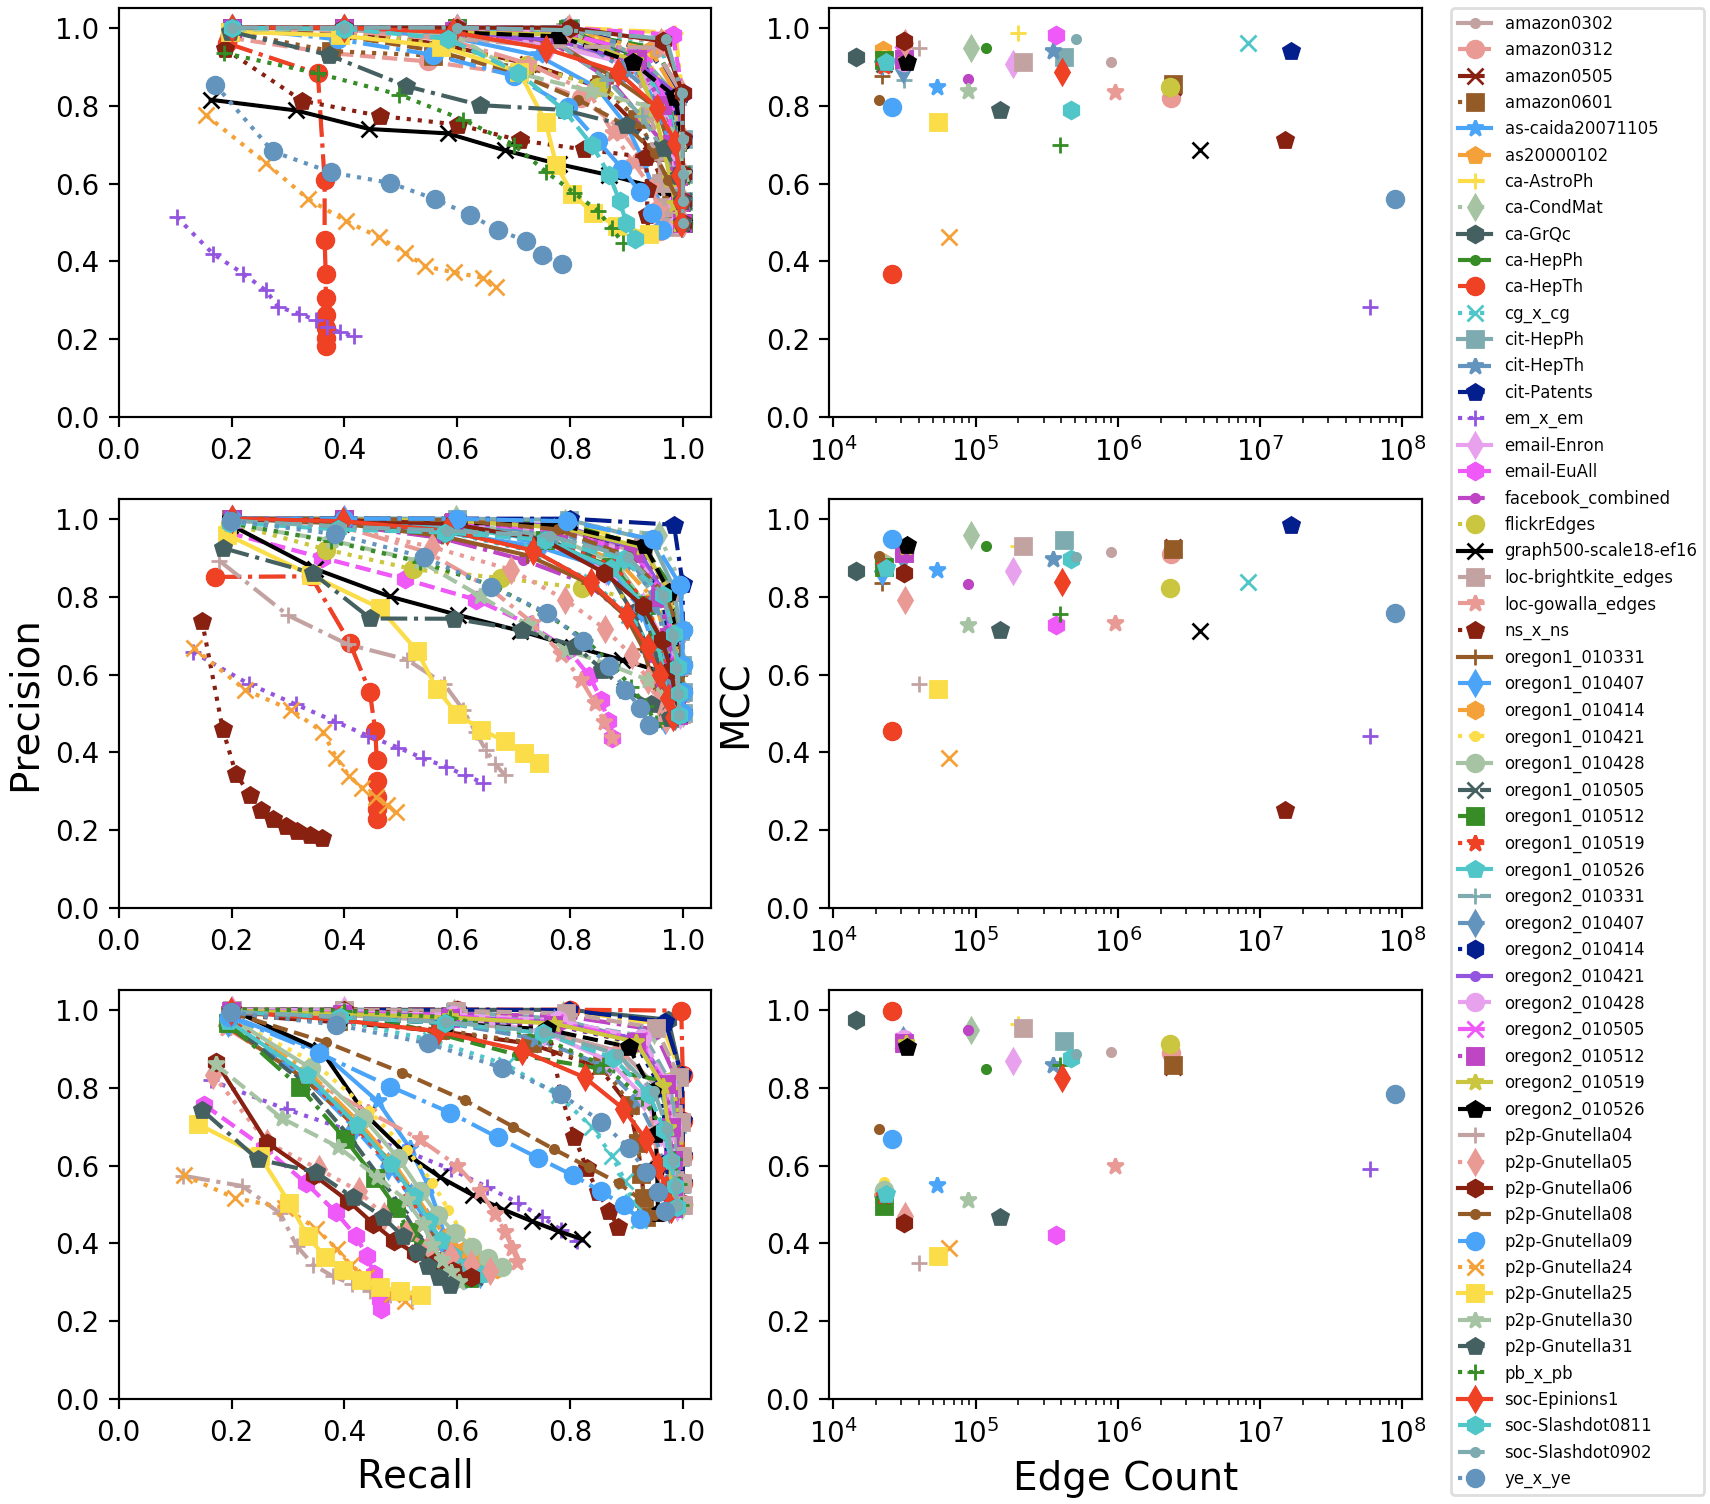
\includegraphics[width=0.7\columnwidth]{precision_vs_recall_all}}

\end{frame}


%----------------------------------------------------------------------------------------

\begin{frame}
\frametitle{Validation of Claims: Relative Error}

\centerline{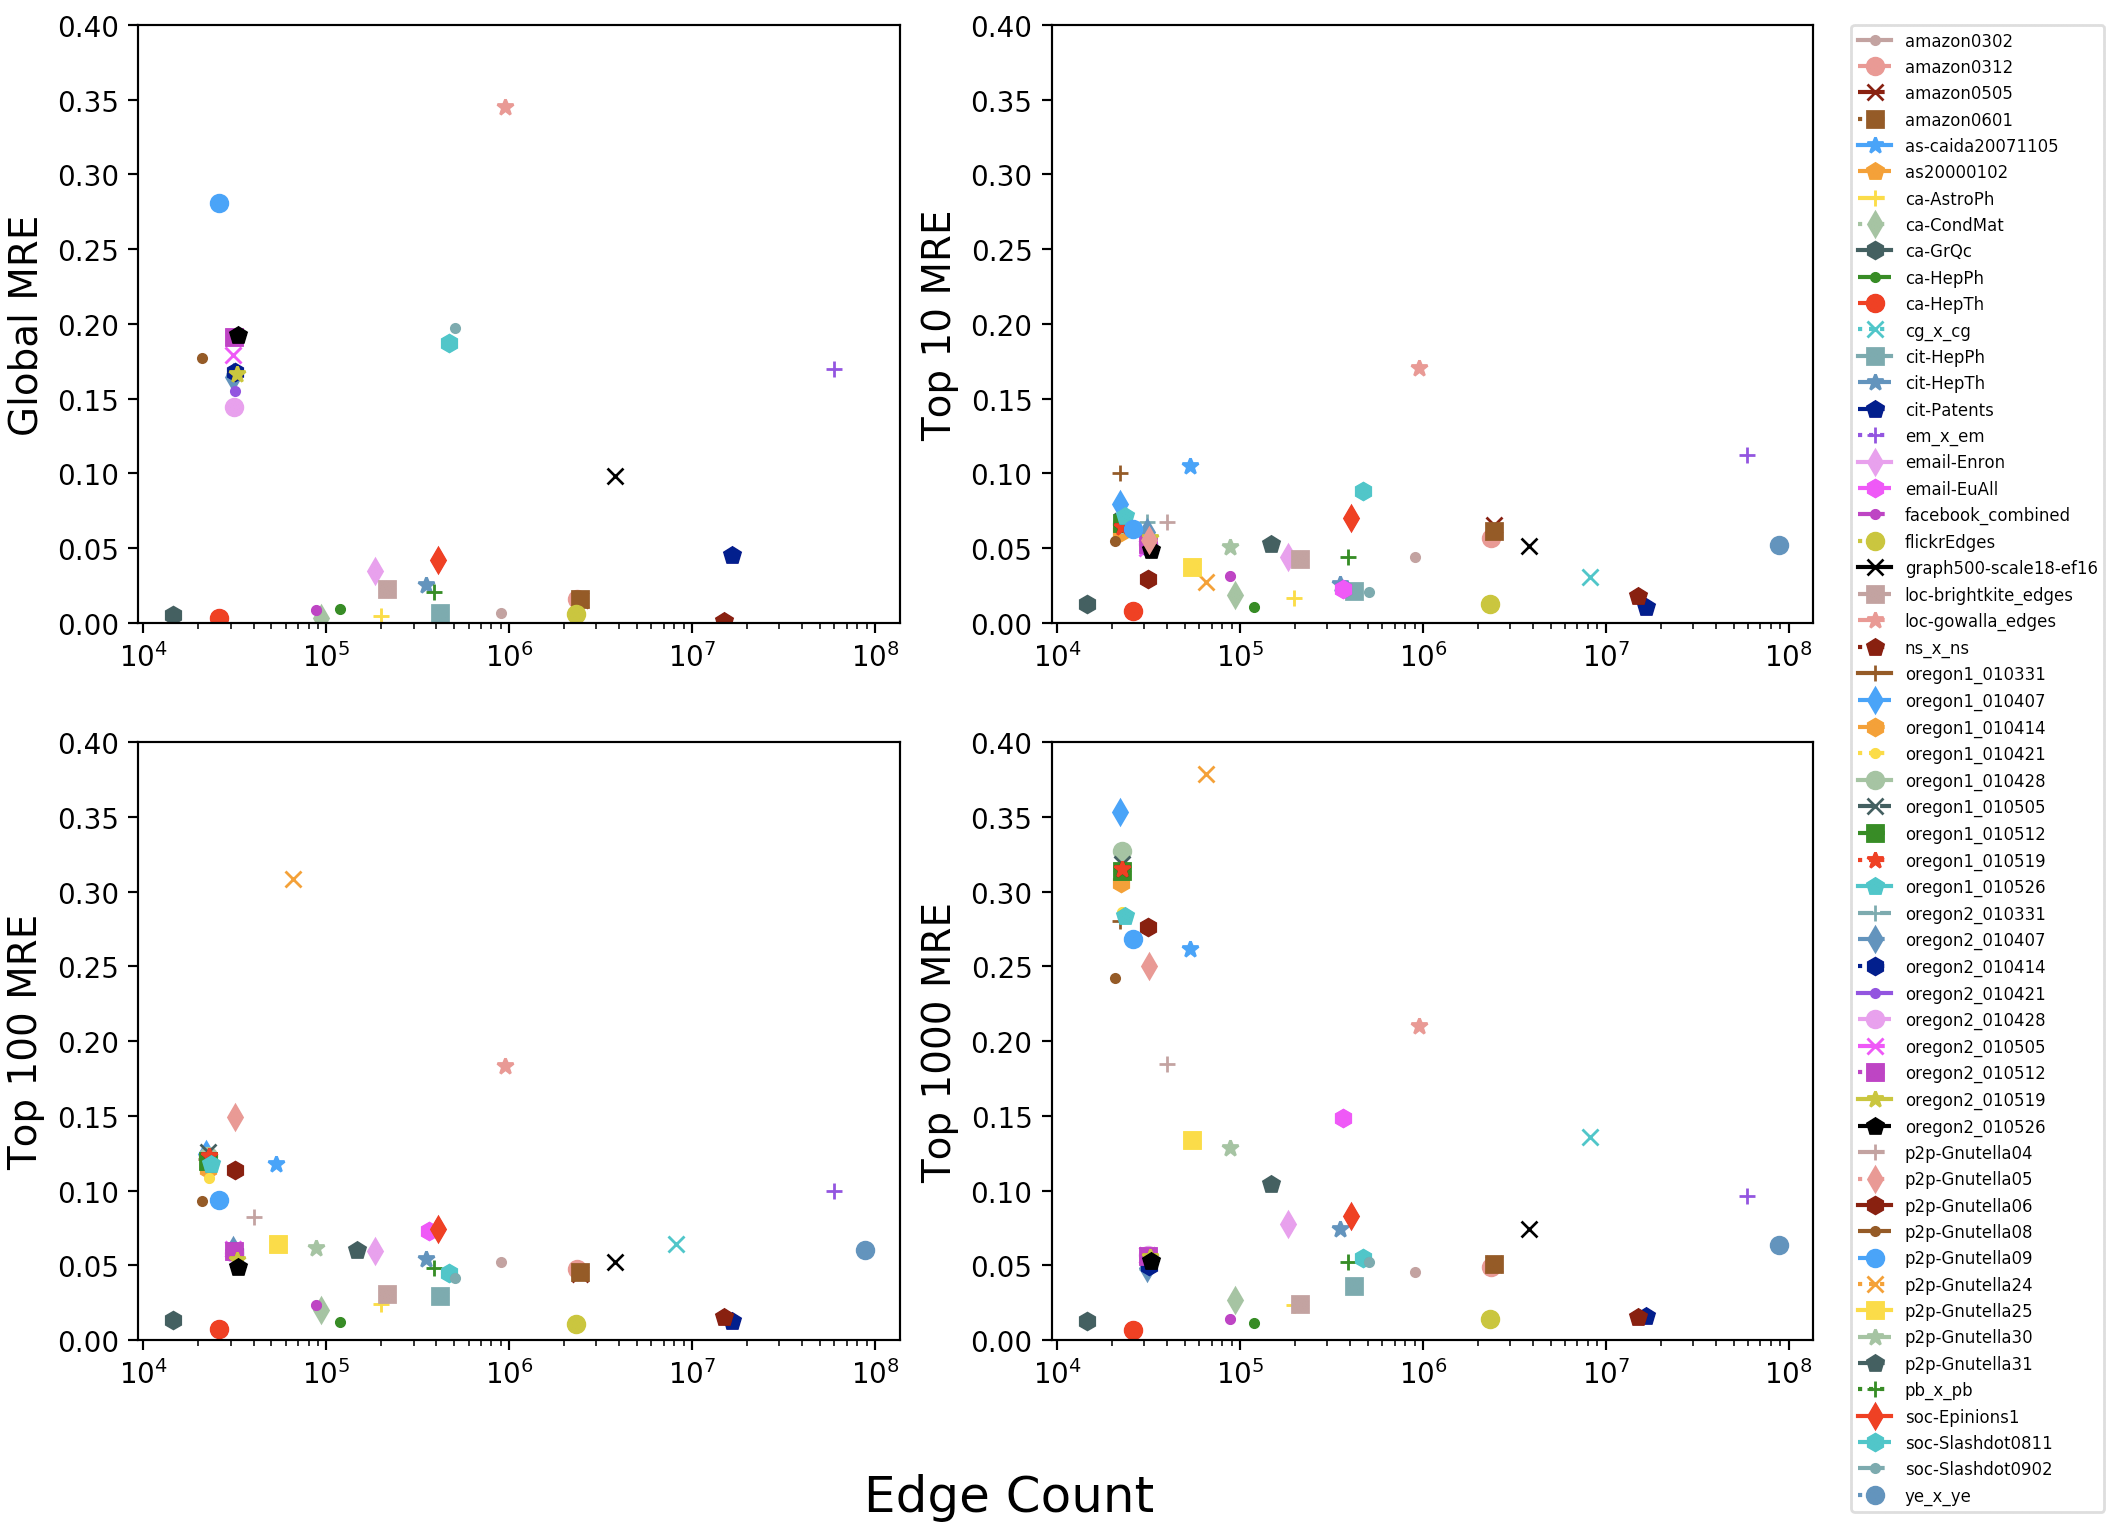
\includegraphics[width=0.9\columnwidth]{errs_vs_E}}

\end{frame}

%----------------------------------------------------------------------------------------

\begin{frame}
\frametitle{Validation of Claims: Good vs Bad Triangle Density}

\centerline{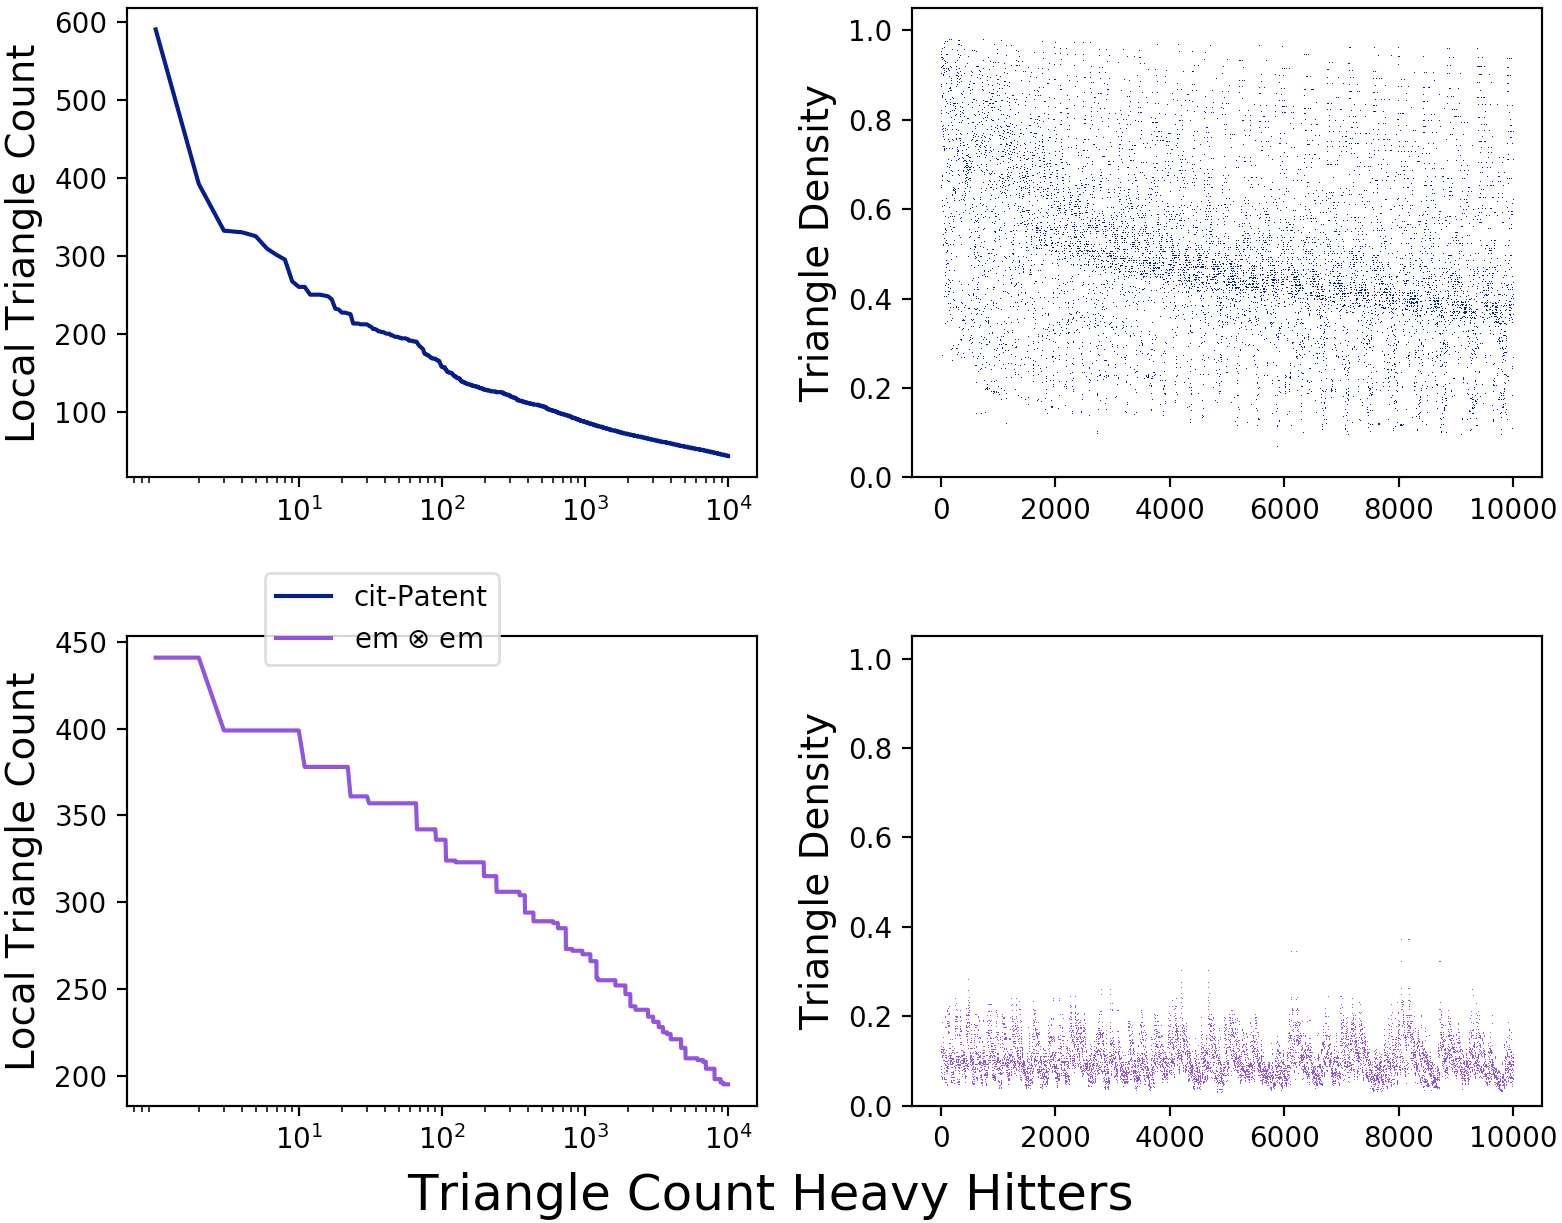
\includegraphics[width=0.8\columnwidth]{hh_comp}}

\end{frame}



%----------------------------------------------------------------------------------------

\begin{frame}
\frametitle{Implementation Details}


\textbf{\algoname{DegreeSketch} C++/MPI Library}
\begin{itemize}
	\item Authored by myself
	\item Utilizes \algoname{YGM} for communication
	\item Accumulation and query API for \algoname{DegreeSketch}
	\item Supports sparse and compressed registers
	\item Implementations for edge- and vertex-local triangle count heavy hitter estimation
	\item Supports more exotic queries
\end{itemize}

\begin{block}{}
	\begin{center}
		\algoname{DegreeSketch} to be open sourced	
	\end{center}
\end{block}

\end{frame}


%----------------------------------------------------------------------------------------
%----------------------------------------------------------------------------------------
\section{Sublinear $\kappa$-Path Centrality}
%----------------------------------------------------------------------------------------
%----------------------------------------------------------------------------------------

\begin{frame}
\frametitle{Motivation: Betweenness Centrality Heavy Hitters}

\textbf{The Problem}:
\begin{itemize}
	\item Computing Betweenness centrality exactly amounts to computing \algoname{AllSourcesAllShortestPaths}
	\begin{itemize}
		\item Expensive $O(mn)$!
	\end{itemize}
\end{itemize}
\textbf{Existing Solutions}:
\begin{itemize}
	\item Approximate via a logarithmic number of \algoname{SingleSourceAllShortestPaths} \cite{green2012fast, bergamini2014approximating, yoshida2014almost, kourtellis2015scalable, riondato2016fast}
	\begin{itemize}
		\item Difficult to distribute
		\item Unclear if possible in $o(m)$ memory
	\end{itemize}
\end{itemize}


\end{frame}



%----------------------------------------------------------------------------------------

\begin{frame}
\frametitle{Approach: Sublinearize $\kappa$-Path Centrality}

\textbf{Idea}: ``Come at the problem sideways''
\begin{itemize}
	\item High $\kappa$-path centrality empirically correlates with high betweenness centrality \cite{kourtellis2013identifying}%[KTSIT13]
	\item Algorithm amounts to sampling random simple paths
	\begin{itemize}
		\item Use $\ell_p$ sampling sketches to sublinearize
	\end{itemize}
	\item Sublinear approximation of $\kappa$-path centrality $\rightarrow$ emprical recovery of high betweenness centrality vertices?
\end{itemize}

\begin{dynblock}
% kappa-path centrality
\opaqueblock<1>{
%
$\kappa$-path centrality
\begin{center}
$\textnormal{PC}(x, \kappa) =  \Pr_{p: |p| \leq \kappa} [x \in p \wedge \text{$p$ a simple path} ]$
\end{center}
%
``simple path'' = non-self-intersecting path
}
\end{dynblock}


\end{frame}



%----------------------------------------------------------------------------------------

\begin{frame}
\frametitle{$\ell_p$ Sampling Sketches}

\begin{dynblock}
% l2 sampling
\opaqueblock<1>{
%
\textbf{$\ell_p$ sampling sketches} \\
Sample from frequency vector $\mathbf{f}$ with probability relative to $\ell_p$ norm
\begin{itemize}
\item Sample $t_i \sim_R (0,1)$ $\forall i \in [n]$
\item Rescale updates to $\mathbf{f}_i$ by $1/t_i^{1/p}$
\item Accumulate \algoname{Tug-of-War}, \algoname{CountSketch}, and $\ell_p$ norm sketches
\item Use sketches to output \algoname{CountSketch} argmax or FAIL
\end{itemize}
%
}
\invblock<2->

% Second block
\opaqueblock<2->[0.4\textwidth]{
%
\vspace{-0.5cm}
%
\begin{center}
Blah blah etc etc\\
It is complex
\end{center}
}
%
\invblock<3->

% Second block
\opaqueblock<3->[0.6\textwidth]{
%
\vspace{-0.5cm}
%
\begin{center}
Outputs $(i,P)$ w.p. $1 - \delta$, where $i \in [n]$ is sampled w.p. $P = (1 \pm \varepsilon)\frac{|v_i|^p}{\|v\|^p_p}$ \cite{monemizadeh20101}
\end{center}
}
%\invblock<3->
%
%% Second block
%\opaqueblock<3->[0.7\textwidth]{
%%
%\vspace{-0.5cm}
%%
%\begin{center}
%$O(\log^2n \log (1/\delta))$ space for $p=0$ \\
%$O(\varepsilon^{-1}\log(1/\varepsilon)\log^2n \log (1/\delta))$ space for $p=1$ \\
%\end{center}
%}

\end{dynblock}



\begin{dynblock}
% rank-k approximation
\opaqueblock<3>{
%
\begin{tabular*}{\textwidth}{l @{\extracolsep{\fill}} r}
\textbf{Useful results}  & \cite{jowhari2011tight, vu2018data}
%[CW09]
\end{tabular*}
%
\vspace{-0.5cm}
%
\begin{itemize}
	\item $\ell_0$ sketch requires $\widetilde{O}(\log (1/\delta))$ memory and update time
	\begin{itemize}
		\item Useful for unweighted random hops
	\end{itemize}
	\item $\ell_1$ sketch requires $\widetilde{O}(\varepsilon^{-1} \log (1/\delta))$ memory and $\widetilde{O}(\log (1/\delta))$ update time
	\begin{itemize}
		\item Useful for weighted random hops
	\end{itemize}
	\item $s$ parallel $\ell_p$ sketches can be accumulated in time independent of $s$
\end{itemize}
}

\end{dynblock}




\end{frame}

%----------------------------------------------------------------------------------------



\begin{frame}
\frametitle{$\ell_p$ Sampling Graph Sparsification}


%\begin{definition}[$\ell_p$-Sampling Sketch]
%A distribution $\Pi$  on $k \times n$ matrices so that if for any $v \in \mathbb{R}^n$, $S$ drawn from $\Pi$ is such that, given $Sv$, one can produce $i \in [n]$ sampled with probability $(1 \pm \varepsilon)\frac{|v_i|^p}{\|v\|_p}$
%\end{definition}

\begin{itemize}
	\item Exploit sketch linearity
	\begin{itemize}
		\item Sample $\ell_0$ sampling sketch matrices $S_1, \dots, S_t$, each of which will sketch every column of $B$
		\item $S_1(B_{:,x})$ returns a sampled neighbor of $x$, say $y$
		\item $S_2(B_{:,x}) + S_2(B_{:,y}) = S_2(B_{:,x} + B_{:,y})$ returns a sampled neighbor of the supervertex $(x + y)$
		\item et cetera
	\end{itemize}
%	\item {[AGM12-1]} \& [AGM12-2] use this method to solve several problems:
	\item This method can solve several problems \cite{ahn2012analyzing, ahn2012graph}:
	\begin{itemize}
		\item $O(n\polylog n)$ to decide connectivity, k-connectivity, bipartiteness, and to approximate the weight of the MST
		\item Multipass $\tilde{O}(n^{1+1/\alpha})$ to compute sparsifiers, the exact MST, \textbf{$\alpha$-spanners}, and approximate the maximum weight matching
	\end{itemize}
\end{itemize}

\begin{block}{}
\begin{center}
We will use similar methods to sample random walks and random simple paths in distributed algorithms
\end{center}
\end{block}

\end{frame}

%----------------------------------------------------------------------------------------



\begin{frame}
\frametitle{Distributed Accumulation $\ell_p$ Sampling Sketches}

%Recall pseudo-asynchronous communication and let $\mathcal{P}$ and $f$ be as before
\begin{itemize}
	\item $P \in \mathcal{P}$ accumulates adjacency set $\mathcal{A}[v]$ for each $v \in \mathcal{V}_P$ %from edge stream
	\begin{itemize}
		\item When $\mathcal{A}[v]$ too large, replace it with $s$ $\ell_0$ sampling sketches
		\item Write current state and all subsequent updates to disk memory % in addition to updating $S_v^{(1)}, \dots, S_v^{(s)}$
	\end{itemize}
	\item Queries to $\mathcal{A}[v]$ return a sampled neighbor of $v$
	\begin{itemize}
		\item If $\mathcal{A}[v]$ is a set of sketches, one is consumed
		\begin{itemize}
			\item If \algoname{Fail}, repeat		
		\end{itemize}
		\item Once $\mathcal{A}[v]$ sketches are exhausted, $P$ takes another pass over $v$'s substream in disk memory
	\end{itemize}
%	\item {[AGM12-1]} \& [AGM12-2] use this method to solve several problems:
\end{itemize}

\begin{block}{}
\begin{center}
Avoids need to subpartition vertices across multiple processors, effectively exchanging communication time for I/O time
\end{center}
\end{block}

\end{frame}

%----------------------------------------------------------------------------------------

\begin{frame}
\frametitle{Sublinear Random Walk and Simple Path Sampling}

\textbf{Random Walk Simulation}
\begin{itemize}
	\item Sample $t$ vertices $\{v_{1,1}, \dots, v_{t,1}\}$ and: 
	\begin{itemize}
		\item Sample $v_{i, j + 1}$ from $\mathcal{A}[v_{i, j}]$
		\item Communicate $(v_{i, 1}, \dots, v_{i, j + 1})$ to $f(v_{i, j + 1})$
%		\item When a processor exhausts $s$ sketches for $v$, take another pass over $a_v$ in disk memory 
	\end{itemize}
\end{itemize}
\textbf{Random Simple Path Simulation}
\begin{itemize}
	\item Similar to random walks, except:
	\begin{itemize}
		\item Do not accumulate sketches ahead of time
		\item Sample $v_{i, j + 1}$ from $\mathcal{A}[v_{i, j}] \setminus \{v_{i, 1}, \dots, v_{i, j - 1}\}$ 
		\begin{itemize}
			\item If $\mathcal{A}[v_{i, j}]$ is not in memory, accumulate a sketch ignoring edges to any of $\{v_{i, 1}, \dots, v_{i, j - 1}\}$
		\end{itemize}
		\item Communicate $(v_{i, 1}, \dots, v_{i, j + 1})$ to $f(v_{i, j + 1})$
	\end{itemize}
\end{itemize}

\begin{block}{}
\begin{center}
Sublinear distributed storage of graph by sketching high degree vertices
\end{center}
\end{block}


\end{frame}

%----------------------------------------------------------------------------------------


\begin{frame}
\frametitle{Sublinear $\kappa$-Path Centrality}

\begin{dynblock}
% kappa-path centrality
\opaqueblock<1>{
$\kappa$-Path Centrality Approximation Algorithm (\cite{kourtellis2013identifying}):
\begin{enumerate}
	\item Simulate $T = 2 \kappa^2 n^{1-2\alpha} \ln n$ $(\leq \kappa)$-length simple paths over $\mathcal{G}$
	\begin{itemize}
		\item maintain $count[x]$ for each $x \in \mathcal{V}$
	\end{itemize}
	\item $\widetilde{\mathcal{C}}^{\kappa}(x) \gets \frac{count[x]}{2 \kappa n^{-2\alpha} \ln n}$
\end{enumerate}
}
%\invblock<2->

%% Second block
%\opaqueblock<2>[0.6\textwidth]{
%%
%\vspace{-0.5cm}
%%
%\begin{center}
%\end{center}
%}

\end{dynblock}


\begin{itemize}
	\item Given $\alpha \in [-1/2,1/2]$, for each $x \in \mathcal{V}$, $\left | \widetilde{\mathcal{C}}^{\kappa}(x) -  \mathcal{C}^{\kappa}(x) \right | \leq n^{1/2+\alpha}$ w.h.p.
	\item Easy to distribute in vertex-centric model
\end{itemize}

%\begin{dynblock}
%% Sublinear kappa-path centrality
%\opaqueblock<3>{
%Sublinear $\kappa$-Path Centrality Approximation Algorithm
%\begin{enumerate}
%	\item Accumulate $\mathcal{A}$ adjacency query structure
%	\item Sample starting vertices $(v_{1,1}, \dots, v_{T,1})$ and lengths $()$Sketch each column of $B$ (node-edge incidence matrix) in parallel over $\kappa$-rounds ($S_{j,1}, \dots, S_{j,T}$ in round $j$)
%	\item Simulate $T$ simple paths as follows, maintaining $count[x]$ as before:
%	\begin{itemize}
%		\item $x_1 \sim V$,
%		\item $x_2 \sim S_{1,i}(x_1)$
%		\item $x_j \sim S_{j,i} \left ( x_{j-1}\right )$, where $S_{j,i}$ is accumulated ignoring edges between $x_{j-1}$ and any of $x_1, \dots, x_{j-2}$
%	\end{itemize}
%	\item $\widetilde{\textnormal{PC}}(x, \kappa) \gets \frac{count[x]}{2 \kappa n^{-2\alpha} \ln n}$
%\end{enumerate}
%}
%\invblock<4->
%
%% Second block
%\opaqueblock<4>[0.8\textwidth]{
%%
%\vspace{-0.5cm}
%%
%\begin{center}
%$T = 2 \kappa^2 n^{1-2\alpha} \ln n$ is a lot of sketches to store \\
%$\kappa$ might be a large number of passes over input
%\end{center}
%}
%%\end{dynblock}
%\invblock<5->
%
%% Second block
%\opaqueblock<5>[0.6\textwidth]{
%%
%\vspace{-0.5cm}
%%
%\begin{center}
%Can we find a sampling algorithm or variant centrality index that affords a sublinear-space approximation of this form?
%\end{center}
%}
%\end{dynblock}



\end{frame}

	
%----------------------------------------------------------------------------------------


\begin{frame}
\frametitle{Sublinear $\kappa$-Path Centrality}

\begin{algorithm}[H]
\caption{Sublinear $\kappa$-Path Centrality}\label{alg:sublinear_kpath}
\begin{algorithmic}[1]
%\State $T \gets 2 \kappa^2 n^{1-2\alpha} \ln n$
\For {$i \in \{1, \dots, T\}$}
	\State $p_i \gets$ empty path
	\State $p_{i,1} \gets$ uniform sample from $\mathcal{V}$
	\State $l_i \gets$ uniform sample from $\{1, 2, \dots, \kappa \}$
\EndFor
\For {$x \in \mathcal{V}$}{$c_x \gets 0$}
\EndFor
\ParFor{$j \in \{1, 2, \dots, \kappa - 1 \}$} 
	\ParFor {$i \in \{1, 2, \dots, T\}$}
		\If {$j < l_i$}
			\State $p_{i,j+1} \gets$ sample from $\mathcal{A}[p_{i,j}]$
			\If {$p_{i,j+1} = \emptyset$}{ discard}
			\EndIf
		\ElsIf {$j = l_i$}
			\State $c_{p_{i,k}} \gets c_{p_{i,k}} + 1$ for $k \in \{1, \dots, j\}$
		\EndIf
	\EndParFor
\EndParFor
\State \Return $c_x /  2 \kappa n^{-2\alpha} \ln n$ for $x \in V$
\end{algorithmic}
\end{algorithm}



\end{frame}





%----------------------------------------------------------------------------------------


%\begin{frame}
%\frametitle{Sublinear Approximation of Dominant Left Eigenvector}
%
%\begin{dynblock}
%% Eigencentrality
%\opaqueblock<1>{
%Eigencentrality
%\begin{itemize}
%	\item Let $A = Q \Lambda Q^{-1}$ be the eigendecomposition of $G$'s adjacency matrix
%	\item $\textnormal{EC}(x) = Q_{1,x}$
%\end{itemize}
%}
%\invblock<2->
%
%% Second block
%\opaqueblock<2>[0.6\textwidth]{
%%
%\vspace{-0.5cm}
%%
%\begin{center}
%Variants: Katz's index, \algoname{PageRank}, \algoname{HITS}, \algoname{SALSA}, \dots
%\end{center}
%}
%\end{dynblock}
%
%
%\begin{dynblock}
%% Question
%\opaqueblock<3->{
%\textbf{Q}: How to sublinearly approximate $Q_{1,:}$?
%%
%\begin{itemize}
%	\item For general square matrices?
%	\item For adjacency matrices of graphs?
%	\item For adjacency matrices of a class of graphs?
%\end{itemize}
%}
%\end{dynblock}
%
%
%
%\begin{dynblock}
%% Answer
%\opaqueblock<4->{
%%
%\textbf{A:} Use low-rank approximations \cite{andoni2013eigenvalues}%[AN13]
%%
%\begin{itemize}
%	\item e.g. sketched SVD-like approximations \cite{sarlos2006improved, clarkson2009numerical, clarkson2017low} or CUR approximations \cite{boutsidis2017optimal}%[DKM06], [DMM08], [BW14] 
%%	\item e.g. sketched SVD-like approximations [S06], [CW09], [CW13] or CUR approximations [DKM06], [DMM08], [BW14] 
%	\item Use factored output $\tilde{A}_k = \tilde{U} \tilde{\Sigma} \tilde{V}^T$ to approximate eigendecomposition
%\end{itemize}
%}
%
%\invblock<5->
%
%% Second block
%\opaqueblock<5>[0.85\textwidth]{
%%
%\vspace{-0.5cm}
%%
%\begin{center}
% Such $\tilde{A}_k$ satisfies $\|A-\tilde{A}_k\|_F \leq (1+\varepsilon) \| A - A_k \|_F$ w.h.p. \\
% There is \textbf{no} guarantee that the approximate singular vectors or that so-constructed eigenvectors will be close to those of $A$
%\end{center}
%}
%
%\end{dynblock}
%
%
%\end{frame}



%----------------------------------------------------------------------------------------


%\begin{frame}
%\frametitle{Sublinear Approximation of Dominant Left Eigenvector}
%
%
%\begin{dynblock}
%% Question
%\opaqueblock<1->{
%\textbf{Q}: So what do we do?
%}
%\end{dynblock}
%
%\begin{dynblock}
%% Answer 1
%\opaqueblock<2->{
%\textbf{A1}: Try it!
%\begin{itemize}
%	\item Low-rank SVD-like approximations still have a lot of $A$'s structure
%	\item May prove empirically useful
%	\item Ennables use of bicriteria solution $AR(SAR)^+SA$ from \cite{clarkson2009numerical}%[CW09]
%	\begin{itemize}
%		\item \textbf{much} faster than true rank-$k$ approximation
%	\end{itemize}
%\end{itemize}
%}
%\end{dynblock}
%
%
%\begin{dynblock}
%% Answer 1
%\opaqueblock<3->{
%\textbf{A2}: Novel algorithms!
%\begin{itemize}
%	\item Bounded-error solution desirable
%	\item Possibly take advantage of structure, like \algoname{HITS} approximation
%	\begin{itemize}
%		\item Limited to graphs, specific classes of graphs, tree width, \dots
%	\end{itemize}
%\end{itemize}
%}
%\end{dynblock}
%
%
%
%\end{frame}



%----------------------------------------------------------------------------------------


%\begin{frame}
%\frametitle{Robustness of Sketches?}
%
%
%\begin{dynblock}
%% Question
%\opaqueblock<1->{
%\textbf{Q}: What happens if there are noisy or malicious updates?
%\begin{itemize}
%	\item Input $v = v^{(g)} + v^{(b)}$
%	\item $S(v) = S(v^{(g)}) + S(v^{(b)})$
%	\item Possible to recover $S(v^{(g)})$ from $S(v)$?
%	\item Overlap during distributed computation?
%\end{itemize}
%}
%\end{dynblock}
%
%
%\begin{dynblock}
%% Answer
%\opaqueblock<2->{
%\textbf{A}: I have no idea
%\begin{itemize}
%	\item I just started thinking about this problem last week
%	\item \cite{hadjieleftheriou2005robust} addresses robustness of distributed sketches
%	\item \cite{hardt2013robust} discusses robustness of \emph{adaptive} streams
%%	\item {[HBK05]} addresses robustness of distributed sketches
%%	\item{[HW13]} discusses robustness of \emph{adaptive} streams
%	\item Certainly important to address for practical implementation
%\end{itemize}
%}
%\end{dynblock}
%
%
%\end{frame}



%----------------------------------------------------------------------------------------


%\begin{frame}
%\frametitle{Implementation and Empirical Evaluation}
%
%\begin{itemize}
%	\item Research goals require empirical evaluation
%	\begin{itemize}
%		\item Disciplined code implementation
%		\item Experiments on real and synthetic data
%		\item Display value of approach to applied community
%	\end{itemize}
%	\item Requires software!
%	\begin{itemize}
%		\item ``Leave-behind'' scientific contribution
%		\item Leverage existing tools
%		\begin{itemize}
%			\item \textbf{libskylark}: Python/C++ sketch library
%			\item \textbf{libelemental}: Python/C++ distributed matrix library
%		\end{itemize}
%	\end{itemize}
%\end{itemize}
%
%
%
%\end{frame}



%----------------------------------------------------------------------------------------


\begin{frame}
\frametitle{Summary of Results}

\begin{itemize}
	\item The Goal: distributed sublinear approximations of centrality indices
	\item Engineering Results
	\begin{itemize}
		\item \algoname{YGM}: Pseudo-Asynchronous 	Communication Handler
	\end{itemize}
	\item Algorithmic Results
	\begin{itemize}
		\item A streaming degree centrality approximation and heavy hitter recovery algorithms
		\item A O(1)-pass semi-streaming closeness centrality approximation algorithm
		\item 2-pass distributed semi-streaming edge- and vertex-local triangle count heavy hitter estimation algorithms using \algoname{DegreeSketch}
		\item Distributed sublinear semi-streaming random walk and random simple path sampling algorithms
		\item Distributed sublinear semi-streaming $\kappa$-path centrality estimation algorithm
	\end{itemize}
	\item Future Work
	\begin{itemize}
		\item Applications for $\algoname{DegreeSketch}$
		\item Sublinear random walk and random simple path implementation
	\end{itemize}
\end{itemize}

\end{frame}


%----------------------------------------------------------------------------------------


\begin{frame}

\begin{center}
{\Huge Questions?}
\end{center}

\end{frame}


%----------------------------------------------------------------------------------------
\nobibliography{../../eed1a7a966f874f4aa88bc8e943e71ce/bibliography.bib} 
\bibliographystyle{alpha} 
%\nobibliography{sketching-centrality} 
%\bibliographystyle{alpha}


\end{document} 